% Document For Use With LuaLaTeX
\documentclass[a4paper,11pt]{article}

% Define Thesis Information
\newcommand{\thesistitle}{Temporal Discretization Based Deviations in Time-Resolved Electron Holography}
\newcommand{\thesisauthor}{Hüseyin Çelik}
\newcommand{\submissiondate}{25\textsuperscript{th} October 2021}

% Fonts and Typography
\usepackage[ngerman,english]{babel}
\usepackage{fontspec,microtype}

% Math and Science
\usepackage[locale=US,per-mode=fraction,separate-uncertainty,sticky-per]{siunitx}
\usepackage[tbtags]{mathtools}
\usepackage{amssymb,physics,interval}

% Bibliography
\usepackage[style=numeric-comp,sorting=none,giveninits=true,doi=false]{biblatex}
\usepackage[nottoc]{tocbibind}
\usepackage{csquotes}

% Layout
\edef\svtheparindent{\the\parindent}
\usepackage[all]{nowidow}
\usepackage{parskip}

% Visuals and Graphics
\usepackage[dvipsnames]{xcolor}
\usepackage{contour,cancel}

% Figures and Captions
\usepackage{graphicx,caption,subcaption,tikz}

% Source Code
\usepackage[cache=false]{minted}

% Links
\usepackage[hidelinks,pdfauthor={\thesisauthor},pdftitle={\thesistitle}]{hyperref}
\usepackage[nameinlink,noabbrev]{cleveref}

% Load After Hyperref
\usepackage[margin=1in]{geometry}
\usepackage{float}

% Enable French Spacing
\frenchspacing

% Add Bibliography File
\addbibresource{References.bib}

% Caption Style
\captionsetup{font=footnotesize,labelfont={bf},belowskip=-11pt}

% Change Source Code Theme
\usemintedstyle{pastie}
\AtBeginEnvironment{minted}{\renewcommand{\colorbox}[3][]{#3}}

% Add TikZ Libraries
\usetikzlibrary{arrows.meta,matrix,decorations.pathreplacing,shapes.geometric,calc,fit}

\begin{document}

\pagenumbering{Alph}
\begin{titlepage}
	\begin{figure}[H]
	\centering
	
\includegraphics[width=0.3\textwidth]{Figures/Logo.pdf}
	\end{figure}
	{\center
	{\LARGE \textsc{Technische Universität Berlin}\\
	\vspace*{10mm}
	\textbf{Faculty II}\\
	Institute of Optics and Atomic Physics}\\
	\vspace*{\fill}

	\hrulefill

	{\Huge \textbf{\thesistitle}\par}

	\hrulefill

	\vspace*{\fill}
	{\LARGE Bachelor Thesis}\\
	\emph{submitted for the degree of Bachelor of Science (B.\,Sc.)}\\
	\vspace*{\fill}
	by\\
	{\Large \textbf{\thesisauthor}}\\
	(Student-No. 0 390 823)\\
	}
	\vspace*{10mm}
	\begin{tabbing}
	\hspace*{4cm}First Examiner: \hspace*{1cm}\=Prof. Dr. Michael Lehmann\\
	\hspace*{4cm}Second Examiner: \>Prof. Dr. Ralph Ernstorfer\\
	\hspace*{4cm}Supervisor: \>Tolga Wagner, M.\,Sc.\\
	\hspace*{4cm}Date of Submission: \>\submissiondate \\
	\end{tabbing}
\end{titlepage}
\newpage

\setcounter{page}{1}
\pagenumbering{roman}

\section*{Declaration of Originality}
I hereby declare that the thesis submitted is my own, unaided work, completed without any unpermitted external help. Only the sources and resources listed were used.

The independent and unaided completion of the thesis is affirmed by affidavit:

\vspace*{1cm}
\hspace*{3.2cm} \includegraphics[scale=0.2]{Figures/Signature.pdf}
\vspace*{-1cm}

\begin{tabular}{@{}p{2cm}p{8cm}@{}}
	\textbf{Signature:} & \hrulefill \\
	& \thesisauthor \\
	& Berlin, \submissiondate \\
\end{tabular}
\newpage
\section*{Abstract}
Time-resolved electron holography, with its separate access to amplitude and phase information of reconstructed electron waves, allows for spatially-resolved sampling of dynamic processes in the nanosecond range. The thereby resulting deviation errors, which are dependent on the temporal resolution and the sampling rate, represent a lower bound error of such time-resolved measurements.

The following thesis presents a self-developed, computer-based method for quantifying these deviation errors. In order to verify its validity, the results obtained by applying the method to three different signal types are compared to experimental measurements. The self-developed method allows for optimizations of the measurement parameters, enabling significant time savings in the measurement process, as well as conclusions on physical properties of sophisticated specimens by means of physical (feedback) modeling.

More precisely, this thesis shows that the deviations arising from the temporal discretization strongly depend on the signal type. For sinusoidal signals, measurement parameters that are within experimental feasibility result in deviations below 1\%, while the same choice of measurement parameters for a complicated Bat-Signal results in deviations of around 5\%. Furthermore, a comparison with an exponential modeling approach for a square wave signal applied to a capacitor shows that the experimentally measured capacitance of the specimen is more applicable to the entire circuit rather than the investigated coplanar capacitor, whose capacitance has to be corrected downwards in the exponential model.
\begin{otherlanguage}{ngerman}
\section*{Deutsche Zusammenfassung}
Die zeitaufgelöste Elektronenholographie, mit ihrem getrennten Zugang zur Amplitude und Phase rekonstruierter Elektronenwellen, ermöglicht die ortsaufgelöste Abtastung dynamischer Prozesse im Nanosekundenbereich. Die aus solch einer Abtastung resultierenden Abweichungsfehler, welche abhängig von der Zeitauflösung und der Abtastrate sind, stellen eine untere Fehlergrenze solcher zeitaufgelösten Messungen dar.

Die folgende Arbeit stellt eine selbst entwickelte, computerbasierte Methode zur Quantifizierung dieser Abweichungsfehler vor. Zu ihrer Verifizierung werden die durch sie gewonnen Ergebnisse für drei verschiedene Signaltypen mit experimentellen Messungen verglichen. Die entwickelte Methode erlaubt eine Optimierung der Messparameter, was zu einer realen Zeitersparnis während des Messprozesses führt, sowie Rückschlüsse auf physikalische Eigenschaften komplexer Proben mittels physikalischer (Feedback-)Modellierung ermöglicht.

Genauer kann in dieser Arbeit gezeigt werden, dass die aus der zeitlichen Diskretisierung entstehenden Abweichungen stark vom Signaltyp abhängen. Für sinusartige Signale ergeben sich bei experimentell sinnvollen Messparametern Abweichungen unter 1\%, während die Abweichungen bei einem komplizierten Bat-Signal für die gleiche Wahl von Messparametern bei ca. 5\% liegen. Ferner kann ein Vergleich mit einem exponentiellen Modellierungsansatz für ein an einem Kondensator angelegten Rechtecksignal zeigen, dass die experimentell gemessene Kapazität der Probe eher auf den gesamten Schaltkreis zutrifft als auf den untersuchten koplanaren Kondensator, dessen Kapazität im exponentiellen Modell nach unten hin korrigiert werden muss.
\end{otherlanguage}
\newpage

\tableofcontents
\newpage

\pagenumbering{arabic}
\setcounter{page}{1}

\section{Introduction} \label{sec:introduction}
With an ever-growing interest in the investigation of dynamic processes at the nanoscale, time-resolved transmission electron microscopy (TEM) is becoming increasingly important. Current stroboscopic approaches yield time resolutions from the nanosecond \cite{Bostanjoglo2000,Doemer2003} down to the femtosecond range \cite{Hassan2017,Zewail2010} while still trying to preserve atomic spatial resolution \cite{Kisielowski2008}. These approaches, however, are not compatible with all modern microscopic techniques used in a TEM. Especially for electron holography, with its separate access to amplitude and phase information of reconstructed electron waves \cite{Lehmann2002,Lichte2007}, making it an excellent candidate for measurements of potential distribution in nanoelectronic devices, these approaches turned out to be very disadvantageous in terms of partial coherence \cite{Feist2017}.

A simple, yet promising novel method, called \emph{interference gating}, avoids these problems and allows for robust time-resolved measurements in electron holography in the nanosecond range by switching the interference pattern on and off \cite{Niermann2017,Wagner2019}. This approach allows for a flexible adjustment of the time window over which the signal is measured, the so called \emph{gate length} $\tau$, and the temporal distance between measurements, the so called \emph{sampling resolution} $t_0$, with minimal additional equipment needed \cite{Niermann2017,Wagner2019}, allowing physical processes to be easily sampled.

Unfortunately, sampling a signal (or process) often introduces a deviation between the original and time-discrete signal, which is dependent on the chosen parameters \cite{Gray1998,Stickler1967,Kobayashi2000}. This thesis introduces a flexible and self-developed approach to quantize this, regardless of experimental setup always present, temporal discretization based deviation in time-resolved electron holography for different kinds of signals and parameters $\tau$ and $t_0$.

In detail, \cref{sec:theoretical-foundations} introduces the theoretical foundations behind electron holography, interference gating and time-discrete signals. \Cref{sec:implementation} first presents the self-developed temporal discretization and deviation evaluation method in order to subsequently discuss its results in an application to a sine wave, square wave and Bat-Signal. \Cref{sec:application} deals with the experimental setup and the time-resolved electron holographic measurements of different input signals applied to an object and discusses the deviations between the aforementioned discretization deviations and measured phase slopes for those signals. At last, \cref{sec:summary-outlook} gives a short summary of the results of this thesis and an outlook on further research in this area.
\newpage
\section{Theoretical Foundations} \label{sec:theoretical-foundations}
This section gives a brief insight into the mathematical and experimental foundations regarding electron holography, interference gating and time-discrete signals.
\subsection{Electron Holography} \label{ssec:electron-holography}
Placing the investigated object such that it is illuminated by a plane electron wave results in a modulation of both the amplitude $a_{obj}\left(\vb{r}\right)$ and the phase ${\varphi}_{obj}\left(\vb{r}\right)$ effecting the object wave ${\psi}_{obj}\left(\vb{r}\right)$ \cite{Lehmann2002,Lichte2007}:
\begin{equation}
	{\psi}_{obj}\left(\vb{r}\right) = a_{obj}\left(\vb{r}\right) e^{i{\varphi}_{obj}\left(\vb{r}\right)}.
\end{equation}
The corresponding wave length\footnote{The wavelength $\lambda = h/p$ of a particle, with its momentum $p$ and the Planck constant $h$, was introduced by Louis de Broglie in 1924 \cite{BrogliePhD1924}.} of the electrons (for an acceleration voltage of $U_a = \SI{300}{\kilo\volt}$ the wave length is $\lambda = \SI{1.97}{\pico\metre}$), which is notably smaller than the atomic structure of the illuminated object, makes this technique a viable microscopy method \cite{Lichte2007,Gabor1948}. In order to realize electron holography, an unmodulated reference wave ${\psi}_{ref}\left(\vb{r}\right)$ needs to propagate through a vacuum region near the illuminated object \cite{Lehmann2002,Lichte2007}. The desired hologram can then be obtained by coherently superimposing both waves, which is achieved by deflecting them with a so called \emph{Möllenstedt biprism} towards each other under an angle $\beta$ (\cref{fig:EH-setup}) \cite{Moellenstedt1956}. The resulting electron hologram $I_{hol}\left(\vb{r}\right)$ (\cref{fig:EH}) follows as \cite{Lehmann2002,Lichte2007}:
\begin{equation}
	I_{hol}\left(\vb{r}\right) = 1 + a^2\left(\vb{r}\right) + 2\mu a\left(\vb{r}\right)\cos(2\pi \vb{q}_c\vb{r} + \varphi\left(\vb{r}\right) + \theta\left(\vb{r},\vb{q}_c\right))
\end{equation}
where $a\left(\vb{r}\right)$ and $\varphi\left(\vb{r}\right) = {\varphi}_{obj}\left(\vb{r}\right) - {\varphi}_{ref}\left(\vb{r}\right)$ are the amplitude and the phase of the reconstructed image wave ${\psi}_{rec}\left(\vb{r}\right)$, $\abs{\vb{q}_c} = {\beta}/{\lambda}$ is the carrier frequency of the interference fringes, $\mu$ is the corresponding contrast \cite{Lehmann2002,Lichte2007} and $\theta\left(\vb{r}, \vb{q}_c\right)$ is an additional phase modulation \cite{LehmannPhD1997}. This yields the important conclusion that the amplitude $a\left(\vb{r}\right)$ results in a contrast modulation (\cref{fig:EH-AMP}) and the phase $\varphi\left(\vb{r}\right)$ in a bending of the interference fringes (\cref{fig:EH-PH}) \cite{Lehmann2002,Lichte2007}.
\begin{figure}[H]
\captionsetup{belowskip=0pt}
	\centering
	\begin{subfigure}[c]{\textwidth}
		\centering
		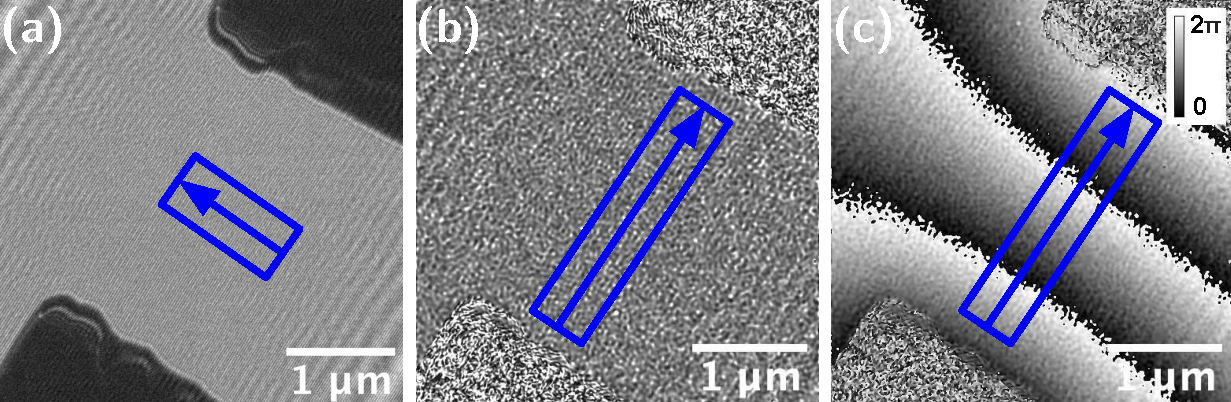
\includegraphics[width=\textwidth]{Figures/Holograms/Holograms.pdf}
	\end{subfigure}
	\hspace{-4mm}
	\begin{subfigure}[c]{0.3\textwidth}
		\centering
		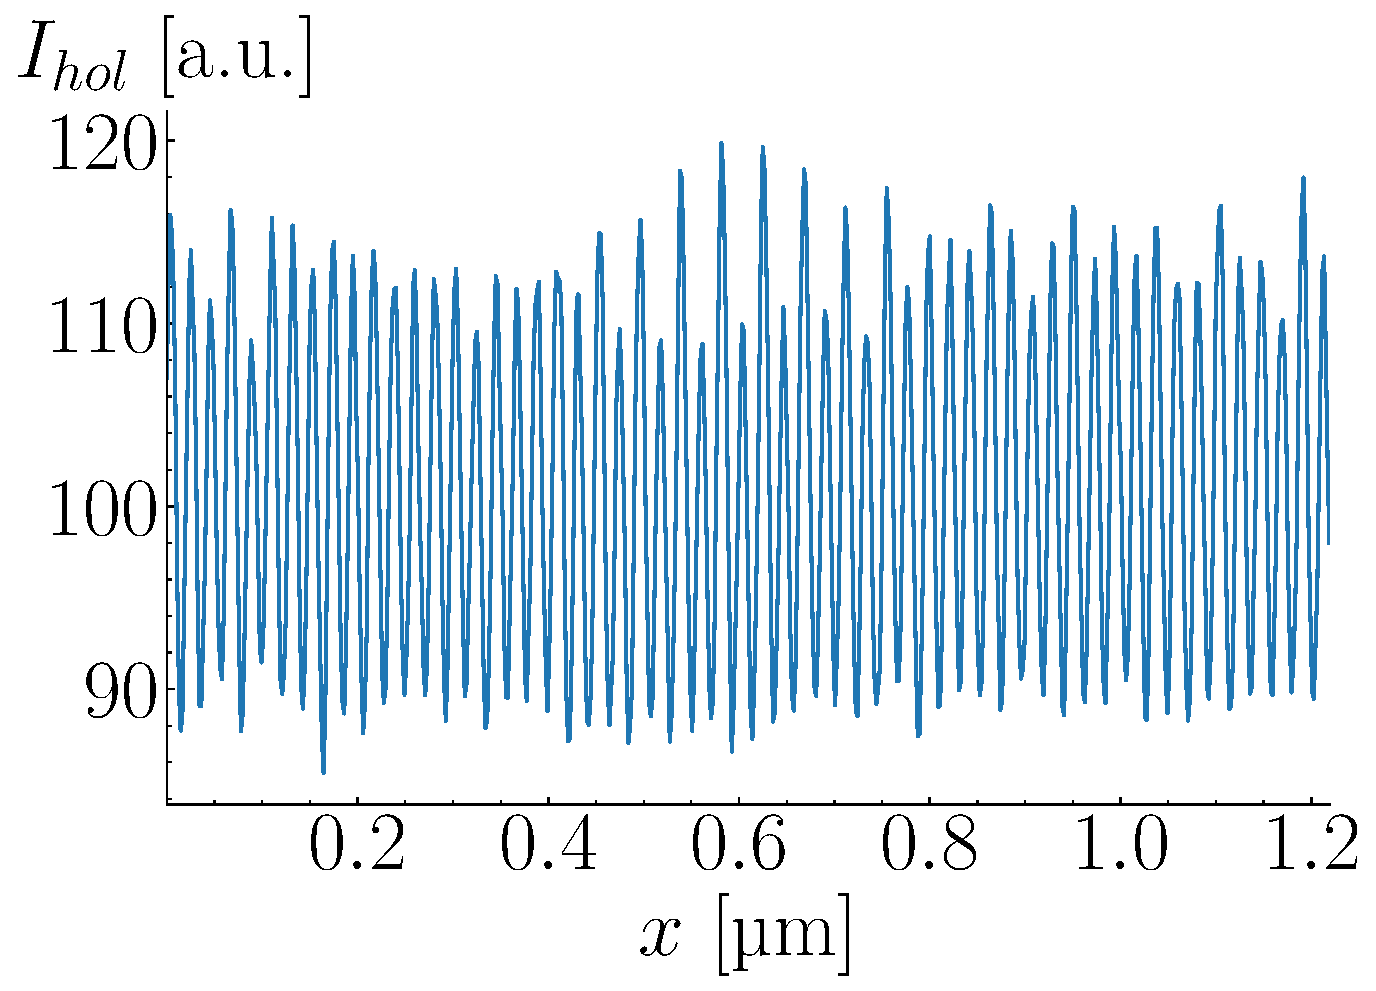
\includegraphics[width=\textwidth]{Figures/Holograms/EH.pdf}
		\phantomsubcaption
		\label{fig:EH}
	\end{subfigure}%
	\hspace{5mm}
	\begin{subfigure}[c]{0.3\textwidth}
		\centering
		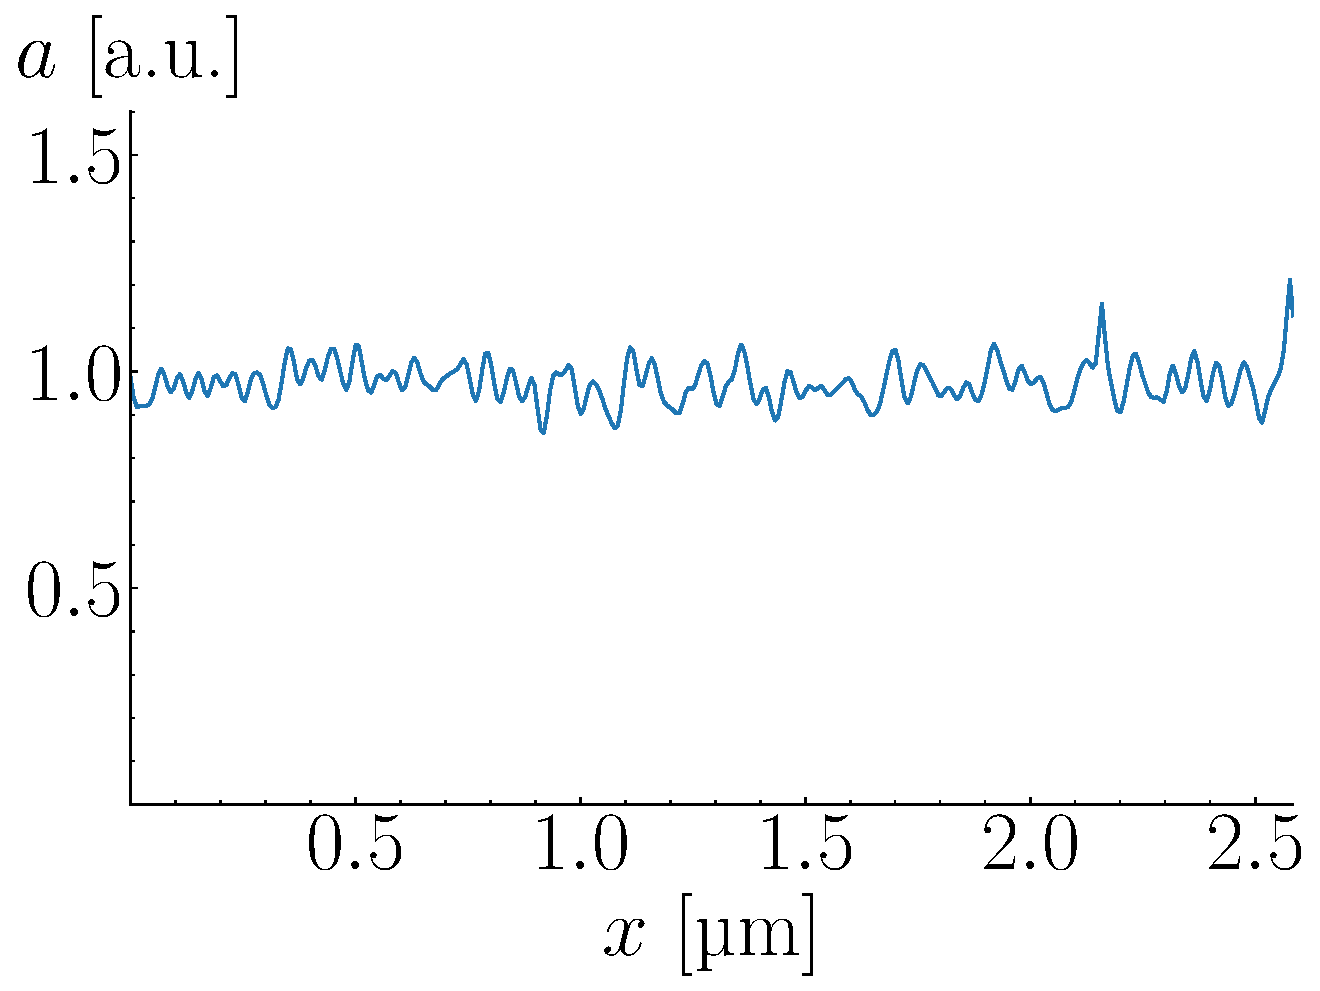
\includegraphics[width=\textwidth]{Figures/Holograms/EH_AMP.pdf}
		\phantomsubcaption
		\label{fig:EH-AMP}
	\end{subfigure}%
	\hspace{4mm}
	\begin{subfigure}[c]{0.3\textwidth}
		\centering
		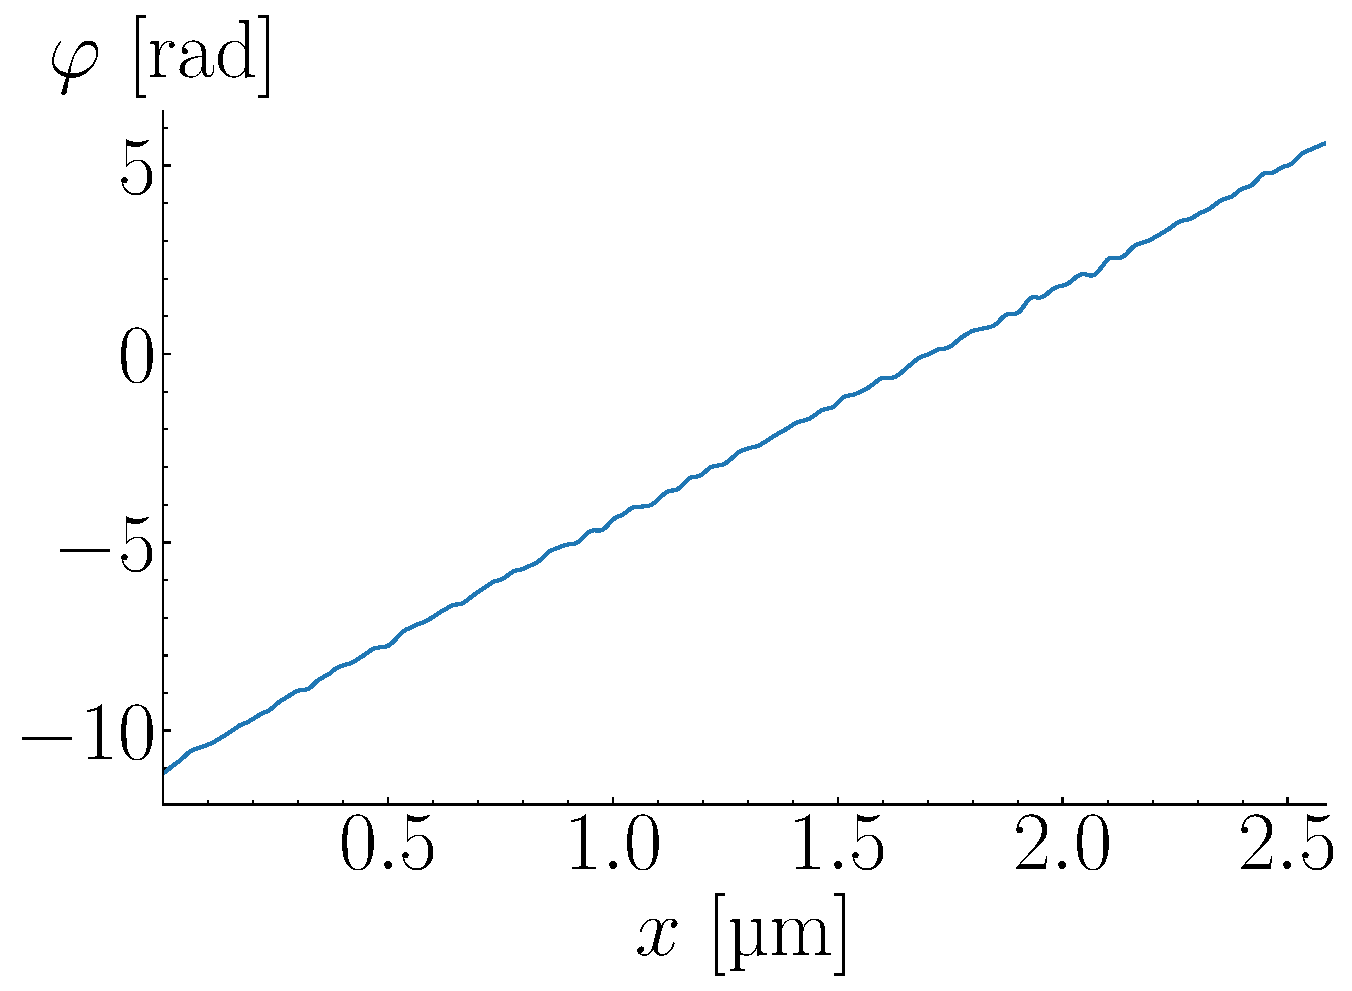
\includegraphics[width=\textwidth]{Figures/Holograms/EH_PH.pdf}
		\phantomsubcaption
		\label{fig:EH-PH}
	\end{subfigure}%
	\caption{Electron holography for a coplanar capacitor biased with $U_{ext} = \SI{1}{\volt}$ with the (a) hologram and its corresponding intensity profile $I_{hol}\left(\vb{r}\right)$, (b) reconstructed amplitude and its corresponding profile $a\left(\vb{r}\right)$ and (c) reconstructed phase and its corresponding unwrapped profile $\varphi\left(\vb{r}\right)$.}
	\label{fig:EH-biased}
\end{figure}
A subsequent Fourier transform of the electron hologram $I_{hol}\left(\vb{r}\right)$ yields \cite{Lehmann1994,Voelkl1995}:
\begin{equation}
	\label{eq:FT-bands}
	\begin{split}
		\mathcal{F}\left\{ I_{hol}\left(\vb{r}\right) \right\} &= \mathcal{F}\left\{ 1 + a^2\left(\vb{r}\right) \right\} \\
		&+ \mu \mathcal{F}\left\{ a\left(\vb{r}\right)e^{i\left(\varphi\left(\vb{r}\right) + \theta\left(\vb{r},\vb{q}_c\right)\right)} \right\} \otimes \delta\left(\vb{q} - \vb{q}_c\right) \\
		&+ \mu \mathcal{F}\left\{ a\left(\vb{r}\right)e^{-i\left(\varphi\left(\vb{r}\right) + \theta\left(\vb{r},\vb{q}_c\right)\right)}\right\} \otimes \delta\left(\vb{q} + \vb{q}_c\right)
	\end{split}
\end{equation}
where the first line of \cref{eq:FT-bands} represents the centerband, the second line the sideband $\left(+1\right)$ and the third line the sideband $\left(-1\right)$ \cite{Lehmann1994,Voelkl1995}. Centering and isolating one of the sidebands in Fourier space allows for the application of an inverse Fourier transform $\mathcal{F}^{-1}$, which in turn leads to the reconstructed image wave ${\psi}_{rec}\left(\vb{r}\right)$ \cite{Lehmann1994,Voelkl1995}:
\begin{equation}
	{\psi}_{rec}\left(\vb{r}\right) = \mu a\left(\vb{r}\right)e^{i\varphi\left(\vb{r}\right)}.
\end{equation}
In order to correct for the various different distortions causing a phase modulation $\theta\left(\vb{r},\vb{q}_c\right)$, an empty hologram is recorded along with every captured object and subtracted from the image phase \cite{voelkl1999,Lichte2007}. Taking the empty hologram $I_{emp}\left(\vb{r}\right)$ immediately after the object holograph results in \cite{voelkl1999}:
\begin{equation}
	I_{emp}\left(\vb{r}\right) = 1 + 2\mu \cos(2\pi \vb{q}_c \vb{r} + \theta\left(\vb{r}, \vb{q}_c\right)).
\end{equation}
If an external bias $U_{ext}$ is applied to the investigated object, therefore modifying its electric potential distribution, a hologram of the unbiased object (i.\,e. $U_{ext} = \SI{0}{\volt}$) can be used as an empty hologram \cite{Niermann2017,Wagner2019}. In doing so, the amplitude $a\left(\vb{r}\right)$ of the reconstructed image wave ${\psi}_{rec}\left(\vb{r}\right)$ is normalized and unwanted phase modulations (e.\,g. induced by surface charging) are automatically subtracted \cite{Wagner2019}.

As an interferometric method, electron holography is susceptible to external disturbances (e.\,g. mechanical vibrations or electromagnetic field fluctuations), requiring a long exposure time of several seconds \cite{Niermann2017}. This limitation imposes special requirements on the coherence properties of the electron source, which has so far limited electron holography to static measurements \cite{Niermann2017}.%
\begin{figure}[H]
	\centering
	\begin{tikzpicture}
	\contourlength{1.5pt}

	\def\centerarc[#1](#2)(#3:#4:#5)[#6][#7]
    {\draw[#1] ($(#2)+({#5*cos(#3)},{#5*sin(#3)})$) arc (#3:#4:#5) node[align=center][#6]{\contour{white}{#7}};}

	\node[rectangle,fill=black!50,draw=black,minimum height=0.75cm,minimum width=0.5cm] (R1) at (0,0) {};
	\node[isosceles triangle,anchor=apex,isosceles triangle apex angle=90,draw=none,rotate=90,fill=black!10,minimum width=3cm] (T1) at (R1.south) {};
	\node[rectangle,fill=black!10,draw=none,minimum height=3cm, minimum width=3cm,anchor=north west] (R2) at (T1.left corner) {};
	\filldraw[fill=black!40,draw=none] (R2.south west) -- (R2.south) -- ++(0,-1.5) -- cycle;
	\filldraw[fill=black!10,draw=none] (R2.south east) -- (R2.south) -- ++(0,-1.5) -- cycle;
	\filldraw[fill=black!30,draw=none] (R2.south west) rectangle (R2.center) node [midway] {${\psi}_{obj}\left(\vb{r}\right)$};
	\filldraw[fill=black!10,draw=none] (R2.center) rectangle (R2.north east) node [midway] {${\psi}_{ref}\left(\vb{r}\right)$};
	\node[rectangle,fill=black!50,draw=black,minimum height=0.2cm,minimum width=1.5cm,ultra thick,anchor=west] (O1) at (R2.west) {};
	\filldraw[fill=black!10,draw=none] ($ (R2.south) + (0,-1.5) $) -- ++(-1,-0.75) -- ++(-0.5,-1.5) -- cycle;
	\filldraw[fill=black!40,draw=none] ($ (R2.south) + (0,-1.5) $) -- ++(1,-0.75) -- ++(0.5,-1.5) -- cycle;
	\filldraw[fill=black!30,draw=none] ($ (R2.south) + (0,-1.5) $) -- ++(-1.5,-2.25) -- ++(3,0) -- cycle;
	\draw[dashdotted] (R1.south) -- ($ (R2.south) + (0,-3.75) $);
	\node[ellipse,fill=black!20,draw=black,minimum height=0.2cm,minimum width=3.5cm,inner sep=0] (E1) at (T1.lower side) {};
	\node[ellipse,fill=black!20,draw=black,minimum height=0.4cm,minimum width=4cm,inner sep=0] (E2) at (R2.south) {};
	\filldraw[fill=black!10,draw=black] ($ (R2.south) + (0,-2.25) $) circle (3pt);
	\node[rectangle,fill=black!50,draw=black,minimum width=0.2cm, minimum height=1cm] (B1) at ($ (R2.south) + (-1.5,-2.25) $) {};
	\node[rectangle,fill=black!50,draw=black,minimum width=0.2cm, minimum height=1cm] (B2) at ($ (R2.south) + (1.5,-2.25) $) {};
	\draw ($ (R2.south) + (-2.5,-3.75) $) -- ++(5,0);
	\node[inner sep=0,align=center,anchor=east] (l1) at ($ (R2.south) + (-2.75,-3.75) $) {Detector};
	\node[inner sep=0,align=center,anchor=east] (l2) at ($ (B1.west) + (-1,0) $) {Biprism};
	\node[inner sep=0,align=center,anchor=east] (l3) at ($ (R2.south) + (-2,-1) $) {Back Focal\\Plane};
	\node[inner sep=0,align=center,anchor=east] (l4) at ($ (E2.west) + (-1,0) $) {Objective};
	\node[inner sep=0,align=center,anchor=east] (l5) at ($ (E1.west) + (-1,0) $) {Condenser};
	\node[inner sep=0,align=center,anchor=east] (l6) at ($ (O1.west) + (-1,0) $) {Object};
	\node[inner sep=0,align=center,anchor=east] (l7) at ($ (R1.west) + (-1,0) $) {Electron\\Source};
	\draw[bend right=30] (l3.east) to ($ (R2.south) + (0,-1.5) $);
	\draw (l2.east) to (B1.west);
	\draw (l4.east) to (E2.west);
	\draw (l5.east) to (E1.west);
	\draw (l6.east) to (O1.west);
	\draw (l7.east) to (R1.west);
	\node[rectangle,fill=black!50,draw=black,minimum width=0.3cm,minimum height=1.5cm] (B3) at (4,-3) {};
	\node[fill=black!50,draw=black,minimum width=0.3cm,minimum height=1.5cm] (B4) at (8,-3) {};
	\draw[ultra thick] (B3.west) -- ++(-0.5,0) -- ++(0,-0.65);
	\draw[ultra thick] ($ (B3.west) + (-0.85,-0.65) $) -- ++(0.7,0);
	\draw[ultra thick] ($ (B3.west) + (-0.75,-0.75) $) -- ++(0.5,0);
	\draw[ultra thick] ($ (B3.west) + (-0.65,-0.85) $) -- ++(0.3,0);
	\draw[ultra thick] (B4.east) -- ++(0.5,0) -- ++(0,-0.65);
	\draw[ultra thick] ($ (B4.east) + (0.85,-0.65) $) -- ++(-0.7,0);
	\draw[ultra thick] ($ (B4.east) + (0.75,-0.75) $) -- ++(-0.5,0);
	\draw[ultra thick] ($ (B4.east) + (0.65,-0.85) $) -- ++(-0.3,0);
	\draw[dotted] ($ (B3.east) + (0,2) $) -- ($ (B4.west) + (0,2) $);
	\draw ($ (B3.east) + (0,-3) $) -- ($ (B4.west) + (0,-3) $);
	\draw[dashdotted] ($ (B3.center) + (2,2) $) -- ($ (B3.center) + (2,-3) $);
	\draw[dotted] (B3.east) -- (B4.west);
	\node[circle,fill=black!30,draw=black,align=center,minimum size=5pt] (C2) at ($ (B3.center) + (2,0) $) {\textbf{+}};
	\draw[ultra thick,dashed] ($ (B3.center) + (2,-3) $) -- ++(70:{3/sin(70)+1.2});
	\draw[ultra thick,dashed] ($ (B3.center) + (2,-3) $) -- ++(110:{3/sin(110)+1.2});
	\draw[ultra thick,<-,>=stealth] ($ (B3.center) + (2,-3) $) -- ++(70:{3/sin(70)});
	\draw[ultra thick,<-,>=stealth] ($ (B3.center) + (2,-3) $) -- ++(110:{3/sin(110)});
	\draw[ultra thick,->,>=stealth] ($ (B3.center) + (2,2) $) -- ++(-60:{2/sin(60)});
	\draw[ultra thick,->,>=stealth] ($ (B3.center) + (2,2) $) -- ++(-120:{2/sin(120)});
	\centerarc[]($ (B3.center) + (2,-3) $)(70:110:1)[midway,below][$\beta$]
	\centerarc[]($ (B3.center) + (2,2) $)(-60:-120:0.8)[midway,above][$\alpha$]
	\centerarc[]($ (B4.center) + (-1,0) $)(65:110:0.8)[midway,below][$\gamma$]
	\draw[<->,>=stealth] ($ (B3.east) + (0.2,2) $) -- node[left] {$a$} ($ (B3.east) + (0.2,0) $);
	\draw[<->,>=stealth] ($ (B3.east) + (0.2,0) $) -- node[left] {$b$} ($ (B3.east) + (0.2,-3) $);
	\node[inner sep=0,align=center,anchor=west] (l1) at ($ (B4.center) + (0,2) $) {Back Focal\\Plane};
	\node[inner sep=0,align=center,anchor=west] (l2) at ($ (B4.center) + (0,-3) $) {Detector};
	\node[inner sep=0,align=center,anchor=west] (l3) at ($ (B3.center) + (4,-4) $) {Hologram};
	\draw[->,>=stealth] ($ (B3.east) + (0,-4.5) $) -- ($ (B4.west) + (0,-4.5) $) node[right] {$x$};
	\draw[->,>=stealth]  ($ (B3.east) + (0,-4.5) $) -- ++(0,1) node[left] {$I_{hol}$};
	\tikzset{shift={(4.23,-7)}}
	\draw[domain=0:9/8*pi,samples=500,smooth,very thick] plot (\x, {sin(8*\x r)*0.4});
\end{tikzpicture}%
	\caption{\emph{Left:} Schematic illustration of the off-axis electron holography process in a TEM \cite{Lehmann2002,Lichte2007}. The electron wave propagates through the object in the left half, creating the modulated object wave ${\psi}_{obj}\left(\vb{r}\right)$, and travels unhindered in the right half, creating the unmodulated reference wave ${\psi}_{ref}\left(\vb{r}\right)$, so they can both be superimposed using a biprism \cite{Lehmann2002,Lichte2007}. \emph{Right:} Schematic illustration representing the deflection of both wave towards each under an angle $\beta$ using a biprism, resulting in a hologram with interference patterns recorded by the detector \cite{Lehmann2002,Lichte2007}.}
	\label{fig:EH-setup}
\end{figure}
\newpage
\subsection{Interference Gating} \label{ssec:igate}
The previously presented electrical biasing electron holography method for investigating electrical potential distributions through electrically biased objects has so far been limited to static measurements \cite{Niermann2017}. In order to also be able to investigate dynamic switching processes, a suitable shutter mechanism, such as the novel interference gating method, is required.

The interference gating method, which uses a destruction of the interference pattern for most of the exposure time $T_{exp}$, enables time-resolved electron holography down to the nanosecond range \cite{Niermann2017,Wagner2019}. If the experimental setup is undisturbed only for a small time period, the so called gate length $\tau$, an interference pattern is able to form during $\tau$ \cite{Niermann2017,Wagner2019}. A temporal shift of the gate length $\tau$, the so called sampling resolution $t_0$, allows for a sampling over the whole period $T$ of a dynamic process (caused by a control signal) \cite{Niermann2017,Wagner2019}.

This destruction of the interference pattern can be described as a dynamic phase shift $\varphi\left(t\right)$, which is easily realized by a voltage variation of the biprism \cite{Niermann2017} or a deflector, causing a slight tilt of the incident beam \cite{Wagner2019}.%
\begin{figure}[H]
	\centering
	\begin{tikzpicture}
	\draw[thick,->,>=stealth] (0,-5) -- (0,0) node[above] {$\varphi$};
	\draw[thick,->,>=stealth] (0,-2.5) -- (6,-2.5) node[right] {$t$};
	\path (0,-5) -- node[left] {$0$} (0,0);
	\path (0,-5) -- (0,-0.5) node[left] {$+\pi$};
	\path (0,0) -- (0,-4.5) node[left] {$-\pi$};
	
	\tikzset{shift={(0,-2.5)}}
	\draw plot[domain=0:5,samples=5000,smooth] (\x, {rand*2});
	\tikzset{shift={(0,2.5)}}
	
	\filldraw[fill=white,draw=none] (2,-5) rectangle (3,0);
	\draw[very thick] (2,-2.5) -- (3,-2.5);
	\draw[<->,>=stealth] (2,-2) -- ++(1,0) node[midway,fill=white] {$\tau$};
	
	\draw[ultra thick,->,>=stealth,red] (4,-0.25) -- ++(0,0.25) -- ++(4,0) -- ++(0,-1.375);
	\draw[ultra thick,->,>=stealth,red] (1,-0.25) -- ++(0,0.75) -- ++(12,0) node[text=black,midway,above] {$\mathcal{F}\left\{ I_{hol}\left(\vb{r},t\right) \right\}$} -- ++(0,-1.875);
	\draw[ultra thick,->,>=stealth,blue] (2.5,-0.25) -- ++(0,0.5) -- ++(8,0) -- ++(0,-1.625);
	
	\filldraw[fill=black,draw=red,ultra thick] (7,-3.5) rectangle (9,-1.5);
	\filldraw[fill=black,draw=blue,ultra thick] (9.5,-3.5) rectangle (11.5,-1.5);
	\filldraw[fill=black,draw=red,ultra thick] (12,-3.5) rectangle (14,-1.5);
	
	\shade[draw=none,shading=radial,inner color=white,outer color=black] (8,-2.5) circle (8pt);
	\shade[draw=none,shading=radial,inner color=white,outer color=black] (10.5,-2.5) circle (8pt);
	\shade[ball color=white,shading=radial,inner color=white,outer color=black] (13,-2.5) circle (8pt);
	\shade[draw=none,shading=radial,inner color=white,outer color=black] (10,-2.5) circle (5pt);
	\shade[draw=none,shading=radial,inner color=white,outer color=black] (11,-2.5) circle (5pt);
	
	\draw[red,thick] (8.5,-2.5) circle (5pt);
	\draw[red,thick] (13.5,-2.5) circle (5pt);
	
	\node[align=center] (l1) at (8,-4.25) {\xcancel{\textbf{Sideband}}};
	\node[align=center] (l1) at (13,-4.25) {\xcancel{\textbf{Sideband}}};
	\node[align=center] (l1) at (10.5,-4.25) {\textbf{Sideband} \checkmark};

\end{tikzpicture}%
	\caption{\emph{Left:} Graph illustrating the dynamic phase shift $\varphi\left(t\right)$ disturbing the hologram except for the gate length $\tau$ \cite{Niermann2017,Wagner2019}. \emph{Right:} Applying the Fourier transform $\mathcal{F}\left\{ I_{hol}\left(\vb{r},t\right) \right\}$ yields only a centerband and no sidebands in Fourier space for the disturbed case, whereas the sidebands are able to form during the gate length $\tau$ \cite{Niermann2017,Wagner2019}.}
	\label{fig:igate}
\end{figure}
The disturbance of the interference patterns causes a loss of holographic information since no sidebands are available in Fourier space (\cref{fig:igate}) \cite{Niermann2017,Wagner2019}. To be precise, disturbing the interference pattern only causes both of the sidebands to disappear in Fourier space, while the centerband remains \cite{Niermann2017,Wagner2019}. If the hologram is captured for the whole duration of the exposure time $T_{exp}$, the above described reconstruction process (\cref{ssec:electron-holography}) acts as a temporal filter on the partially disturbed (time-resolved) hologram, therefore only retaining the information acquired during the undisturbed gate length $\tau$ \cite{Niermann2017,Wagner2019}.

To combat the worsened signal-to-noise ratio caused by a reduction of the fringe contrasts, which is dependent on the so called \emph{gate fraction} $\tau / T$, multiple periods $T$ as well as multiple holograms of the same reversible measurement are averaged \cite{Niermann2017,Wagner2019}. With this, interference gating can be conducted in a pump-probe manner \cite{Mueller2014,Bothschafter2009} for the investigation of periodic processes, which can be externally controlled by a dynamic input voltage $U_{ext}\left(t\right)$ acting as the so called \emph{input signal} \cite{Niermann2017,Wagner2019}. Sampling such periodic processes always results in a temporal discretization, which is described in detail in \cref{ssec:discrete-signals}.
\newpage
\subsection{Time-Discrete Signals} \label{ssec:discrete-signals}
Given an aperiodic and Lebesgue integrable function $g\left(t\right) \in L^1\left(\mathbb{R}^n\right)$, the Fourier transform $\hat{g}\left(f\right)$ is defined as \cite{rahman2011,kaiser2011}:
\begin{equation}
	\hat{g}\left(f\right) = \int_{-\infty}^{\infty} g\left(t\right) e^{-2\pi i f t} \dd{t} = \mathcal{F}\left\{g\left(t\right)\right\}.
\end{equation}
The Fourier transform can thus be considered a transformation from the time domain $t$ to the frequency domain $f$ \cite{rahman2011,kaiser2011}.

Along with the Fourier transform, there exists an inverse Fourier transform, resulting in a Fourier transform pair, defined as \cite{rahman2011,kaiser2011}:
\begin{equation}
	g\left(t\right) = \int_{-\infty}^{\infty} \hat{g}\left(f\right) e^{2\pi i f t} \dd{f}.
\end{equation}

The simplest approach to sample a continuous signal $g\left(t\right)$ is the \emph{ideal sampling} with the sampling period $t_0$, where $g\left(t\right)$ is multiplied by the Dirac comb \cite{engelberg2008,ceschi2017}:
\begin{equation}
	{\Delta}_{t_0} \left(t\right) \coloneqq \sum_{n = -\infty}^{\infty} \delta\left(t - n \cdot t_0\right)
\end{equation}
resulting in the sampled signal \cite{engelberg2008,ceschi2017}:
\begin{equation}
	g_s\left(t\right) = g\left(t\right) \cdot {\Delta}_{t_0} = g\left(t\right) \sum_{n = -\infty}^{\infty} \delta\left(t - n \cdot t_0\right) = \sum_{n = -\infty}^{\infty}g\left(n \cdot t_0\right)\delta\left(t - n \cdot t_0\right).
\end{equation}
The Fourier series of the sampled signal $g_s\left(t\right)$ thus follows as \cite{engelberg2008,ceschi2017}:
\begin{equation}
	\hat{g}_s\left(f\right) = \hat{g}\left(f\right) * \left[\frac{1}{t_0} \sum_{n = -\infty}^{\infty}\delta\left(f - \frac{n}{t_0}\right)\right]
\end{equation}
where $*$ denotes the convolution of two functions \cite{engelberg2008,ceschi2017}. The frequency spectrum of the sampled signal $g_s\left(t\right)$ is therefore the frequency spectrum of the signal $g\left(t\right)$ repeated with period $1/t_0$ and an amplitude scaled to $1/t_0$. Multiplying this spectrum with a rect function of width $1/t_0$ yields the spectrum $\hat{g}\left(f\right)$ \cite{engelberg2008,ceschi2017}.

Real world limitations, such as the impossibility to generate ideal Dirac impulses, make the above approach non feasible, requiring a new approach: The so called \emph{sample and hold}. Here, the Dirac comb is replaced with a rect function of width $T_{rect}$, which is equivalent to a convolution with the rect function \cite{engelberg2008,ceschi2017}:
\begin{equation} \label{eq:sample-and-hold-time}
	g_s\left(t\right) = \sum_{n = -\infty}^{\infty} g\left(n \cdot t_0\right) \cdot \text{rect}\left(\frac{t - n \cdot t_0}{T_{rect}}\right) = \text{rect}\left(\frac{t}{T_{rect}}\right) * \sum_{n = -\infty}^{\infty} g\left(t\right)\delta\left(t - n \cdot t_0\right)
\end{equation}
where the $\text{rect}\left(t\right)$ function is defined as \cite{engelberg2008,ceschi2017}:
\begin{equation}
\text{rect}\left(t\right) \coloneqq
\begin{cases*}
1 & if $\abs{t} \leq \frac{1}{2}$ \\
0 & otherwise
\end{cases*}.
\end{equation}
The resulting frequency spectrum is the frequency spectrum from the ideal sampling approach weighted with a factor containing the sinc function \cite{engelberg2008,ceschi2017}:
\begin{equation} \label{eq:sample-and-hold-frequency}
	\hat{g}_s\left(f\right) = T_{rect} \cdot \text{sinc}\left(f \cdot T_{rect}\right) \cdot \left[\hat{g} * \frac{1}{t_0}\sum_{n = -\infty}^{\infty}\delta\left(f - \frac{n}{t_0}\right)\right].
\end{equation}

The \emph{Nyquist-Shannon sampling theorem} states that a signal $g\left(t\right)$ bearing a band limit $f_{max}$ can be exactly reconstructed using a sampling frequency of $2 \cdot f_{max}$ \cite{Shannon1949}.

If, in contrast to the sample and hold method, the input signal is averaged over an extended discretization interval, additional attenuation occurs in the frequency domain, which is reflected in the time domain in a deviation between the time-discrete and input signal. In the following \cref{sec:implementation}, a self-developed method is presented to quantify this deviation for different temporal discretization parameters $\tau$ and $t_0$.

\newpage
\section{Temporal Discretization and Deviation Evaluation} \label{sec:implementation}
While the previous \cref{sec:theoretical-foundations} dealt with the theoretical foundations surrounding electron holography, interference gating and time-discrete signals, this section, as the main focus of this thesis, details the self-developed method and its various steps to discretize the input signal and evaluate its deviation. This approach provides a quantification of the discretization deviation generally introduced by time resolved measurements like the interference gating method.

The self-developed method can be broken down into two main sections (\cref{fig:flowchart}): While the first part deals with the actual temporal discretization of the input signal (\cref{ssec:discretization-method}), the second part evaluates the deviation between the time-discrete and input signal (\cref{ssec:evaluation-method}).

The temporal discretization step (\cref{fig:flowchart}) is designed in accordance to the interference gating method such that the arbitrary input signal (corresponding to the control signal) is averaged over defined time intervals (corresponding to the gate length $\tau$) at different equidistant time points (corresponding to the sampling resolution $t_0$). The resulting deviations depend (as described in \cref{ssec:discrete-signals}) on the temporal discretization parameters $\tau$ and $t_0$ and are quantified in the evaluation part (\cref{fig:flowchart}). The self-developed method allows for predictions to be made about an appropriate choice of measurement parameters $\tau$ and $t_0$ for time-resolved measurements using interference gating for different control signals.%
\begin{figure}[H]
	\centering
	\begin{tikzpicture}
	\tikzstyle{startstop} = [rectangle,rounded corners,minimum width=3cm,minimum height=1cm,text centered,draw=none,fill=blue!30,align=center]
	\tikzstyle{error} = [ellipse,minimum width=3cm,minimum height=1cm,text centered,draw=none,fill=red!30,align=center]
	\tikzstyle{process} = [rectangle,minimum width=3cm,minimum height=1cm,text centered,draw=none,fill=orange!30,align=center]
	\tikzstyle{decision} = [trapezium,trapezium left angle=70,trapezium right angle=110,minimum width=3cm,minimum height=1cm,text centered,draw=none,fill=green!30,align=center]

	\matrix[matrix of nodes, nodes in empty cells, column sep=0.6cm, row sep=1cm, anchor=center, nodes={anchor=center}]{
	\node (start) [startstop] {Input Data}; &
	\node (split) [process] {Split Data}; &
	\node (length) [decision] {Intervals \\ Equally Sized?}; &
	\node (average) [process] {Average \\ Intervals};\\
	& & \node (warning) [error] {Output \\ Warning}; & \\
	\node (average-dev) [startstop] {Normalize Average \\ Deviation}; &
	\node (calc-dev) [process] {Calculate Single \\ Deviations}; &
	\node (spline-data) [process] {Input Data \\ into Spline}; &
	\node (spline) [process] {Construct \\ Cubic Spline};\\};
	\draw [thick,->,>=stealth] (start) -- (split);
	\draw [thick,->,>=stealth] (split) -- (length);
	\draw [thick,->,>=stealth] (length) -- node[left] {\textsc{no}} (warning);
	\draw [thick,->,>=stealth] (length) -- node[below] {\textsc{yes}} (average);
	\draw [thick,->,>=stealth] (warning) -- (average);
	\draw [thick,->,>=stealth] (average) -- (spline);
	\draw [thick,->,>=stealth] (spline) -- (spline-data);
	\draw [thick,->,>=stealth] (spline-data) -- (calc-dev);
	\draw [thick,->,>=stealth] (calc-dev) -- (average-dev);
	\draw [ultra thick, draw=cyan, fill=white, fill opacity=0, rounded corners] (-7.8,-1.2) rectangle (7.8,3.2);
	\draw [ultra thick, draw=magenta, fill=white, fill opacity=0, rounded corners] (-7.8,-3.2) rectangle (7.8,-1.4);
	\node [text=cyan] (l1) at (0,3.5) {\textbf{Temporal Discretization}};
	\node [text=magenta] (l2) at (0,-3.5) {\textbf{Deviation Evaluation}};
\end{tikzpicture}%
	\caption{Flowchart outlining the various steps of the temporal discretization and deviation evaluation method. The flowchart can be broken down into two main sections: The first part (outlined in cyan) deals with the actual discretization of the input signal by splitting it into equally sized intervals and averaging over them, whereas the second part (outlined in magenta) evaluates the deviation between the time-discrete signal and the input signal at every data point by means of a cubic spline interpolation.}
	\label{fig:flowchart}
\end{figure}
Even though various different methods for comparing, and especially evaluating the deviation between, different signals have been developed throughout the years, most approaches are only optimized for certain types of signals under certain restrictions and yield subpar results otherwise \cite{Bellman1959,Flores1986,Makridakis1993,Elmore2001,Hyndman2006,Kennedy2007,Kim2016}. To be precise, these methods are either unsuitable for signals of different length or sampling resolution, cannot be applied to signals that feature values that are (near) zero or are confined to non-intuitive or limited scales \cite{Bellman1959,Flores1986,Makridakis1993,Elmore2001,Hyndman2006,Kennedy2007,Kim2016}.

The presented method addresses these kinds of problems by applying a more generalized approach suitable for a wide range of signals without imposing unnecessary constrains. In detail, the use of cubic spline interpolation allows for the comparison of signals with non-matching and arbitrary lengths or sampling resolutions, while normalizing the deviation to the peak-to-peak amplitude avoids undefined cases or numerical instability. 
\subsection{Temporal Discretization Method} \label{ssec:discretization-method}
The temporal discretization step of the self-developed method is intended to emulate the measurement process of time-resolved techniques (e.\,g. interference gating). In contrast to the sample and hold method described in \cref{eq:sample-and-hold-time}, this approach averages over a time interval $\tau$ instead of simply locking at a constant value.

The temporal discretization of the input signal is achieved in multiple steps. Starting with the input signal $U\left(t\right)$ as a set of $k$ discrete data points, both the time values $t_i$ and the voltage values $U_i$, with $i \in \mathbb{N}$ and $i \leq k$, are split in equally\footnote{If the chosen combination of interval size and interval spacing leads to non-integer sized intervals, the last interval is truncated in such a manner that the specified parameters can still be realized and the user is warned.} sized intervals, representing the gate length $\tau$, with equal spacing, representing the sampling resolution $t_0$, in between. Those intervals are then averaged, leading to $n$ time-discrete data points $\overline{U}_j\left(t_{g_j}\right)$ for $n$ intervals (\cref{fig:discretization-method}). If the time values $t_i$ are all uniformly sampled, the averaged time $t_{g_j}$ is just the median of the current interval.

This approach poses one problem: Selecting a gate length $\tau$ that is large relative to the period length $T$ (e.\,g. $\tau = 0.5T$) would position the first time-discrete data point far into the signal, effectively truncating the interpolated time-discrete signal, and therefore the domain for the deviation evaluation, compared to the input signal. This means that comparing both signals would be limited to the length of the shorter interpolated time-discrete signal. In order to circumvent this restriction, the signal is artificially extended to multiple periods, or the input signal that is provided is already of sufficient length, and time discretized and interpolated over those multiple (at least three) periods. The deviation between both signals is then only evaluated at a single period $T$ that is not the first or last one, effectively extending the domain for the deviation evaluation to a full period $T$ of the input signal, including the edges.%
\begin{figure}[H]
	\centering
	\begin{tikzpicture}[domain=0:2.2*pi, samples=500, scale=1.9, smooth]
	\draw [thick,->,>=stealth] (0,0) -- (2.4*pi,0) node[right] {$t$ $\left[\si{\second}\right]$};
	\draw [thick,->,>=stealth] (0,-1.3) -- (0,1.3) node[above] {$U$ $\left[\si{\volt}\right]$};
	\filldraw [fill=blue!10,draw=black] (2/8*pi, 0) rectangle (4/8*pi, {sin(3/8*pi r)*0.8});
	\draw [red] plot (\x, {sin(\x r)});
	\draw [decorate,decoration={brace,amplitude=5pt,mirror,raise=5pt}]
	(2/8*pi,0) -- (4/8*pi,0) node[midway,yshift=-20pt]{$t_{g_j}$};
	\draw [decorate,decoration={brace,amplitude=5pt,mirror,raise=5pt}]
	(4/8*pi,0.05) -- (4/8*pi,{sin(3/8*pi r)*0.8-0.05}) node[midway,xshift=20pt]{$\overline{U}_j$};
	\node (l1) at (5/8*pi,1.25) {$\overline{U}_j\left(t_{g_j}\right)$};
	\node[text=red] (l2) at (2.2*pi,0.8) {$U\left(t\right) = U_0 \cdot \sin(\omega t)$};
	\node [fill=black,circle,inner sep=0pt,outer sep=0pt, minimum size=4pt] (c1) at (3/8*pi,{sin(3/8*pi r)*0.8}) {};
	\draw[dashed] (2/8*pi, 0) -- (2/8*pi, -0.8);
	\draw[dashed] (4/8*pi, 0) -- (4/8*pi, -0.8);
	\draw[dashed] (2*pi, -1.25) -- (2*pi, 0);
	\draw[dashed] (7/8*pi,{sin(7/8*pi r)*0.8}) -- (7/8*pi,-0.8);
	\draw[dashed] (9/8*pi,{sin(9/8*pi r)*0.8}) -- (9/8*pi,-0.8);
	\draw[<->,>=stealth] (2/8*pi, -0.8) -- (4/8*pi, -0.8) node [midway, fill=white] {$\tau$};
	\draw[<->,>=stealth] (7/8*pi, -0.8) -- (9/8*pi, -0.8) node[midway,fill=white] {$t_0$};
	\draw[<->,>=stealth] (0, -1.25) -- (2*pi, -1.25)  node [midway, fill=white] {$T$};
	\draw[->,>=stealth,bend angle=30,bend right] (l1.west) to node {} ([yshift=1pt] c1.north);
	\filldraw (1/8*pi,{sin(1/8*pi r)*0.8}) circle (1pt);
	\filldraw (3/8*pi,{sin(3/8*pi r)*0.8}) circle (1pt);
	\filldraw (5/8*pi,{sin(5/8*pi r)*0.8}) circle (1pt);
	\filldraw (7/8*pi,{sin(7/8*pi r)*0.8}) circle (1pt);
	\filldraw (9/8*pi,{sin(9/8*pi r)*0.8}) circle (1pt);
	\filldraw (11/8*pi,{sin(11/8*pi r)*0.8}) circle (1pt);
	\filldraw (13/8*pi,{sin(13/8*pi r)*0.8}) circle (1pt);
	\filldraw (15/8*pi,{sin(15/8*pi r)*0.8}) circle (1pt);
\end{tikzpicture}%
	\caption{Graph illustrating the temporal discretization of the input signal $U\left(t\right)$: The input signal is averaged, both in time $t_{g_j}$ and voltage $\overline{U}_j$, resulting in time-discrete data points $\overline{U}_j\left(t_{g_j}\right)$. The width of the interval represent the gate length $\tau$, the distance between them the sampling resolution $t_0$.}
	\label{fig:discretization-method}
\end{figure}
This approach allows for a flexible adjustment of both the gate length $\tau$ and the sampling resolution $t_0$, thus preserving the implementation of the interference gating method detailed in \cref{ssec:igate}, while still being suitable for a wide range of signals. Furthermore, averaging over both the time $t$ and the voltage $U$ takes into account the trend of the signal over the whole interval, unlike the sample and hold method described in \cref{eq:sample-and-hold-time} that only considers the signal at a single point $t_i$ in time.

Depending on the discretization parameters $\tau$ and $t_0$, this results in inherent deviations from the input signal, which affect the accuracy of real measurements (e.\,g. interference gating) when investigating dynamic processes. In the deviation evaluation step (\cref{ssec:evaluation-method}), these deviations are quantified in order to subsequently make a suitable choice of parameters $\tau$ and $t_0$.
\subsection{Deviation Evaluation Method} \label{ssec:evaluation-method}
In order to evaluate the deviation between the time-discrete data points from the previous step and the input signal, the $n$ time-discrete data points are interpolation with a cubic spline $S$ \cite{Dyer2001}, resulting in the interpolated time-discrete signal $U_S\left(t\right)$ (\cref{fig:evaluation-method}). This method allows for a comparison at every time point $t_i$ of the input signal while still guaranteeing that \cite{Dyer2001}:
\begin{itemize}
	\item The reconstructed curve goes through all $n$ time-discrete data points, the so called \emph{knots}, therefore satisfying $S\left(t_{g_j}\right) = \overline{U}_j$.
	\item The $n$ knots are connected by $n-1$ piecewise cubic polynomials, avoiding problems such as \emph{Runge's phenomenon} \cite{Runge1901}.
	\item The resulting spline $S \in C^2$ is twice continuously differentiable by requiring that the first and second derivatives $S'_l\left(t_{g_j}\right) = S'_{l-1}\left(t_{g_j}\right)$ and $S''_l\left(t_{g_j}\right) = S''_{l-1}\left(t_{g_j}\right)$ match for all $n$ knots, resulting in a function that is smooth at all points, including where two polynomials meet.
\end{itemize}
Furthermore, cubic spline interpolation in the time domain $t$ leads to lower deviations than nearest neighbour and linear interpolation \cite{Hussain2015} while avoiding ringing effects encountered in sinc interpolation through zero padding in the frequency domain $f$ \cite{Yaroslavsky1996}. Additionally, the use of cubic spline interpolation allows the self-developed method to be independent of temporal offsets of the input signal.

The reason for interpolating the $n$ time-discrete data points instead of directly comparing them with the input signal can be shown with a simple example:

Setting the gate length $\tau$ to a single data point, thus not actually averaging over an interval but simply picking the corresponding value in the input signal, while setting the sampling resolution to $t_0 = 0.5T$ of the period length $T$ would yield a deviation of zero, even though only two data points can hardly describe non-sinusoidal signal perfectly.%
\begin{figure}[H]
	\centering
	\begin{tikzpicture}[domain=0:2.2*pi, samples=500, scale=1.9, smooth]
	\draw [thick,->,>=stealth] (0,0) -- (2.4*pi,0) node[right] {$t$ $\left[\si{\second} \right]$};
	\draw [thick,->,>=stealth] (0,-1.3) -- (0,1.3) node[above] {$U$ $\left[\si{\volt}\right]$};
	\draw[dashed] (2*pi, -1.25) -- (2*pi, 0);
	\draw[<->,>=stealth] (0, -1.25) -- (2*pi, -1.25)  node [midway, fill=white] {$T$};
	\draw [red] plot (\x, {sin(\x r)});
	\draw [green] plot (\x, {sin(\x r)*0.8});
	\node[text=red] (l1) at (2.2*pi,0.8) {$U\left(t\right) = U_0 \cdot \sin(\omega t)$};
	\node[anchor=north west,text=green] (l2) at (1/4*pi,0.5) {$U_S\left(t\right)$};
	\node[text=blue] (l3) at (9/8*pi,0.8) {$d_{t_i} = \abs{U\left(t_i\right) - U_S\left(t_i\right)}$};
	\foreach \x in {0.1875,0.25,...,0.8125}{
		\draw [ultra thin, <->, >=stealth, blue] ({\x*pi},{sin(\x*pi r)*0.8}) -- ({\x*pi},{sin(\x*pi r)});}
	\foreach \x in {1.1875,1.25,...,1.8125}{
		\draw [ultra thin, <->, >=stealth, blue] ({\x*pi},{sin(\x*pi r)*0.8}) -- ({\x*pi},{sin(\x*pi r)});}
				\filldraw (1/8*pi,{sin(1/8*pi r)*0.8}) circle (1pt);
	\filldraw (3/8*pi,{sin(3/8*pi r)*0.8}) circle (1pt);
	\filldraw (5/8*pi,{sin(5/8*pi r)*0.8}) circle (1pt);
	\filldraw (7/8*pi,{sin(7/8*pi r)*0.8}) circle (1pt);
	\filldraw (9/8*pi,{sin(9/8*pi r)*0.8}) circle (1pt);
	\filldraw (11/8*pi,{sin(11/8*pi r)*0.8}) circle (1pt);
	\filldraw (13/8*pi,{sin(13/8*pi r)*0.8}) circle (1pt);
	\filldraw (15/8*pi,{sin(15/8*pi r)*0.8}) circle (1pt);
\end{tikzpicture}%
	\caption{Graph illustrating the deviation evaluation between the interpolated time-discrete signal $U_S\left(t\right)$ and input signal $U\left(t\right)$: The time-discrete data points $\overline{U}_j\left(t_{g_j}\right)$ are interpolated with a cubic spline $S$, so the resulting absolute difference $d_{t_i}$ between both signals can be calculated at every time point $t_i$.}
	\label{fig:evaluation-method}
\end{figure}
After interpolating the $n$ time-discrete data points with a cubic spline, all input time values $t_i$ can be input into the spline, allowing to calculate the absolute deviation $d_{t_i} = \abs{U\left(t_i\right) - U_S\left(t_i\right)}$ between the interpolated time-discrete signal $U_S\left(t\right)$ and the input signal $U\left(t\right)$ at every time point $t_i$. In order to give an intuitive, single measurement of the deviation, all absolute deviations $d_{t_i}$ are summed up and averaged, yielding: $$\overline{d} = \frac{1}{k}\sum^k_{i=1}d_{t_i}.$$ 
To ensure easy comparability between different signals, the averaged absolute deviation $\overline{d}$ can be normalized to the peak-to-peak amplitude $U_{pp} = \abs{U_{max}-U_{min}}$, resulting in: $$\overline{d}_{pp} = \frac{\overline{d}}{U_{pp}}.$$ 
This approach, unlike those mentioned at the beginning of \cref{sec:implementation}, does not suffer from flaws such as being undefined for values that are zero, placing heavier penalties on negative deviations than on positive deviations, having a maximum deviation of 100\%, yielding extremely high deviations for small values or being confined to a non-intuitive or limited scale \cite{Bellman1959,Flores1986,Makridakis1993,Elmore2001,Hyndman2006,Kennedy2007,Kim2016}.
\subsection{Discretization and Evaluation of Real Signals} \label{ssec:real-signals}
A particular advantage of the self-developed method is its universal application to various types of input signal. Moreover, like the investigation of physical processes, which can feature various types of dynamics (e.\,g. linear, quadratic, exponential), the generalized approach of the self-developed method allows for the investigation of different input signals.

The following subsection discusses the results from the above described method for three different signals: a sine wave, a square wave and a Bat-Signal. All $m$ deviations $\overline{d}_{pp}$, with $m$ denoting the number of possible combinations of gate length $\tau$ and sampling resolution $t_0$, which are provided relative to the period length $T$ of the respective signal, are normalized to the peak-to-peak amplitude $U_{pp}$ as specified in \cref{ssec:evaluation-method}.
\subsubsection{Sine Wave Signal} \label{sssec:sine-wave}
Starting with a sine wave signal, an exemplary plot showcasing the temporal discretization method can be seen in \cref{fig:sine-real-i2000-s1000}. Here, the gate length of $\tau = 0.2T$ is represented by the light blue bars, which overlap due to the choice of sampling resolution $t_0 = 0.1T$. 
\begin{figure}[H]
	\centering
	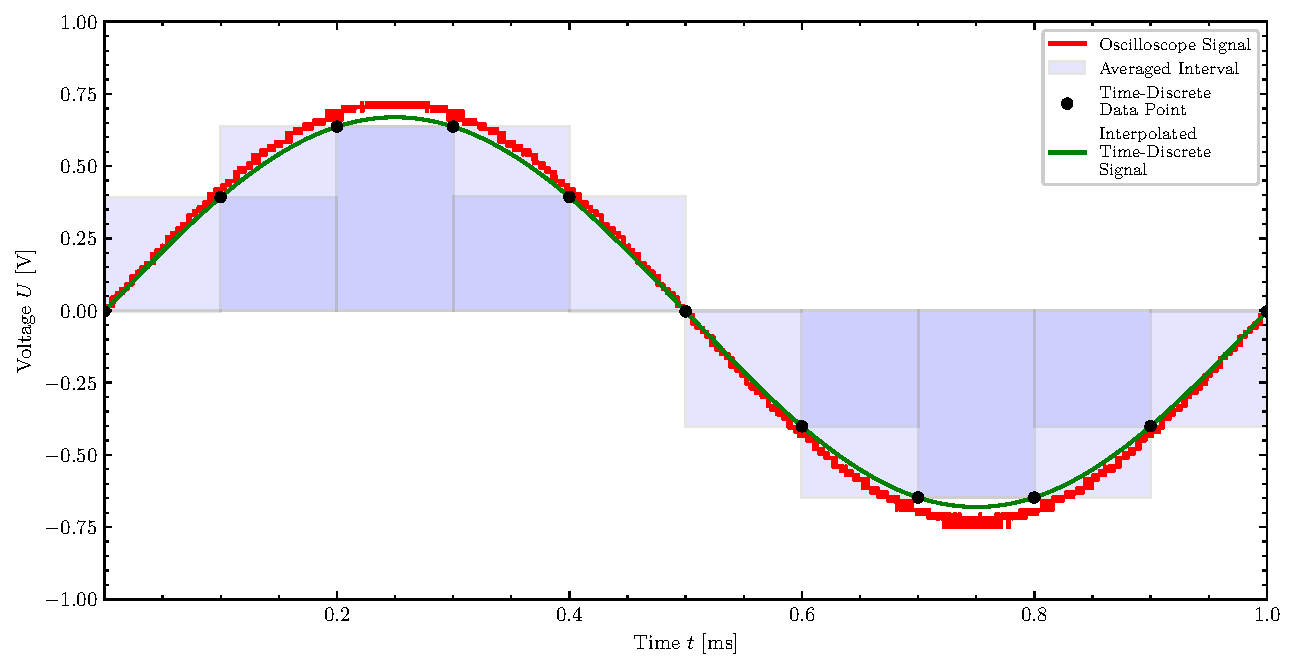
\includegraphics[width=0.75\textwidth]{Figures/Signals/sine_real_i2000_s1000.pdf}
	\caption{Plot of the oscilloscope sine wave signal $U\left(t\right)$ along with the (overlapping) intervals over whom are averaged, the time-discrete data points $\overline{U}_j\left(t_{g_j}\right)$ and the interpolated time-discrete signal $U_S\left(t\right)$ for a gate length of $\tau = 0.2T$ and a sampling resolution of $t_0 = 0.1T$.}
	\label{fig:sine-real-i2000-s1000}
\end{figure}
Both the gate length $\tau$ and the sampling resolution $t_0$ can subsequently be set to values in an interval of $\tau, t_0 \in \interval[scaled, open left]{0}{0.5T}$, where $m$, the number of possible combinations, depends on the chosen step size of $\tau$ and $t_0$. The $m$ different deviations $\overline{d}_{pp}$ can then be calculated and plotted in two dimensions (\cref{fig:sine-real-combination}), revealing two interesting conclusions:
\begin{itemize}
	\item In order to achieve a deviation of $\overline{d}_{pp} < 5\%$, both the gate length $\tau$ and the sampling resolution $t_0$ can be set to values up to $\tau = t_0 \approx 0.3T$.
	\item A gate length of $\tau = 0.1T$ and a sampling resolution of $t_0 = 0.05T$, which is easily within experimental feasibility, yield a deviation of $\overline{d}_{pp} < 1\%$.
\end{itemize}
This shows that signals which do not feature rapid changes in amplitude or slope over small intervals can be sampled with gate lengths $\tau$ and sampling resolutions $t_0$ beyond $0.1T$ while still resulting in a time-discrete signal that is representative of the oscilloscope signal (i.\,e. low single digit deviation $\overline{d}_{pp}$).
\begin{figure}[H]
	\centering
	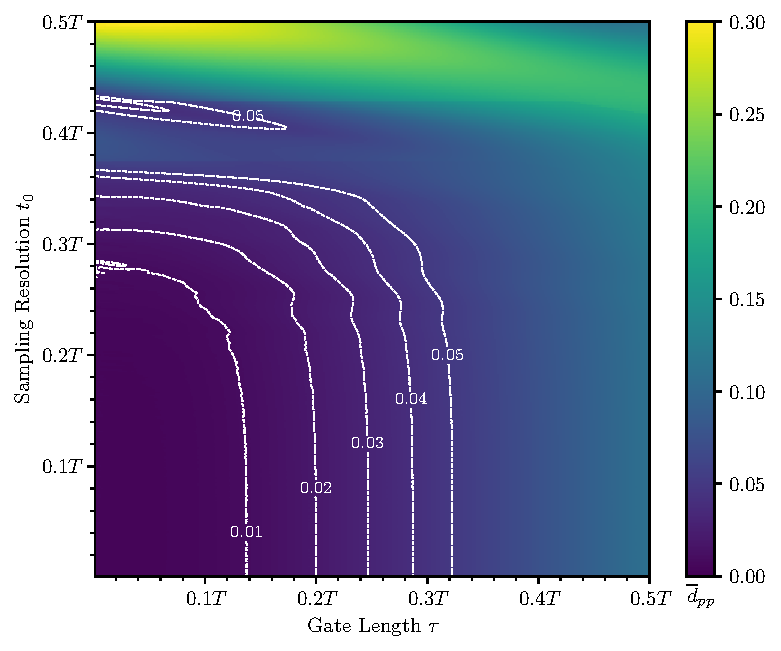
\includegraphics[width=0.5\textwidth]{Figures/Combinations/sine_real.pdf}
	\caption{Two-dimensional plots showcasing the $m$ different deviations $\overline{d}_{pp}$ of the sine wave signal for different combinations of gate length $\tau$ and sampling resolution $t_0$, where both parameters are set to $\tau, t_0 \in \interval[scaled, open left]{0}{0.5T}$, with dashed contour lines for $\overline{d}_{pp} = 0.01, \dotsc ,0.05$.}
	\label{fig:sine-real-combination}
\end{figure}
It should be noted that setting the gate length close to one sampling point while choosing a sampling resolution of $t_0 = 0.5T$ leads to a deviation of $\overline{d}_{pp} > 30\%$, which is reflected in the yellow artifact region in \cref{fig:sine-real-combination}. This is caused by the fact that such a small gate length $\tau$ is effectively equivalent to the corresponding value in the oscilloscope signal, which is (near) zero for a sine wave signal and a sampling of resolution of $t_0 = 0.5T$. The resulting time-discrete data points are therefore all (near) zero as well, yielding an interpolated time-discrete signal that is effectively a straight line of slope zero. Lowering the sampling resolution to just $t_0 = 0.4T$ mitigates most of this since the intervals are now positioned at non-zero values for the sine wave signal.
\subsubsection{Square Wave Signal} \label{sssec:square-wave}
Switching from a sine wave to a square wave signal (\cref{fig:square-real-i50-s25}), the same two dimensional plot showcasing the deviation $\overline{d}_{pp}$ of $m$ different combinations of gate length $\tau$ and sampling resolution $t_0$ can be calculated (\cref{fig:square-real-combination}). This shows that the same deviation of $\overline{d}_{pp} < 5\%$ requires a gate length of $\tau < 0.15T$ and a sampling resolution of $t_0 < 0.1T$. Furthermore, a gate length of $\tau = 0.1T$ and sampling resolution of $t_0 = 0.05T$, which is easily within experimental feasibility, results in a deviation of $\overline{d}_{pp} \approx 3\% - 4\%$, three to four times that of the sine wave signal.

Examining \cref{fig:square-real-i50-s25}, for which a gate length of $\tau = 0.1T$ and sampling resolution of $t_0 = 0.05T$ was used, reveals that, even-though the deviation $\overline{d}_{pp}$ is two to three times higher than the sine wave signal, the interpolated time-discrete signal is still an accurate representation of the oscilloscope square wave signal.
\begin{figure}[H]
	\centering
	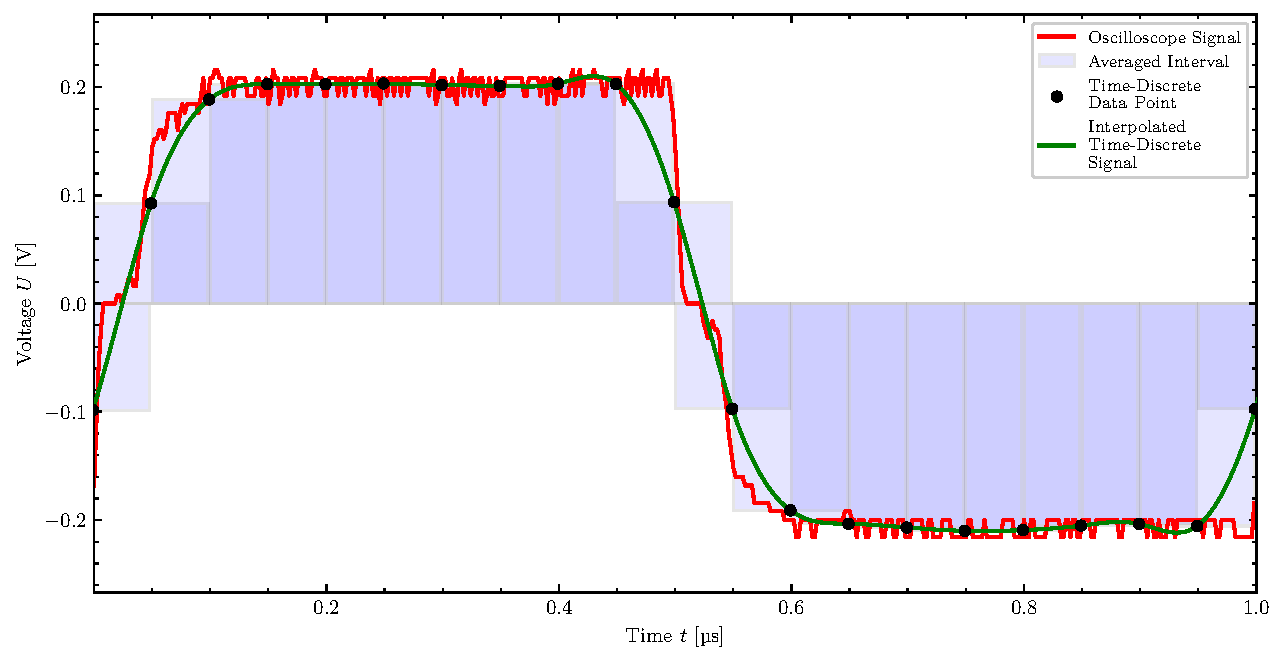
\includegraphics[width=0.75\textwidth]{Figures/Signals/square_real_i50_s25.pdf}
	\caption{Plot of the oscilloscope square wave signal $U\left(t\right)$ along with the (overlapping) intervals over whom are averaged, the time-discrete data points $\overline{U}_j\left(t_{g_j}\right)$ and the interpolated time-discrete signal $U_S\left(t\right)$ for a gate length of $\tau = 0.1T$ and a sampling resolution of $t_0 = 0.05T$.}
	\label{fig:square-real-i50-s25}
\end{figure}
A large contribution to the deviation $\overline{d}_{pp}$ stems from not only the noise of the oscilloscope signal causing small deviations at every data point, but also from the sections of sharp rise and fall in both signals. Nevertheless, pushing the gate length $\tau$ and sampling resolution $t_0$ both beyond $0.15T$ quickly results in two digit deviations $\overline{d}_{pp}$, a sharp contrast to the observations of the sine wave signal from \cref{sssec:sine-wave}.
\begin{figure}[H]
	\centering
		\centering
	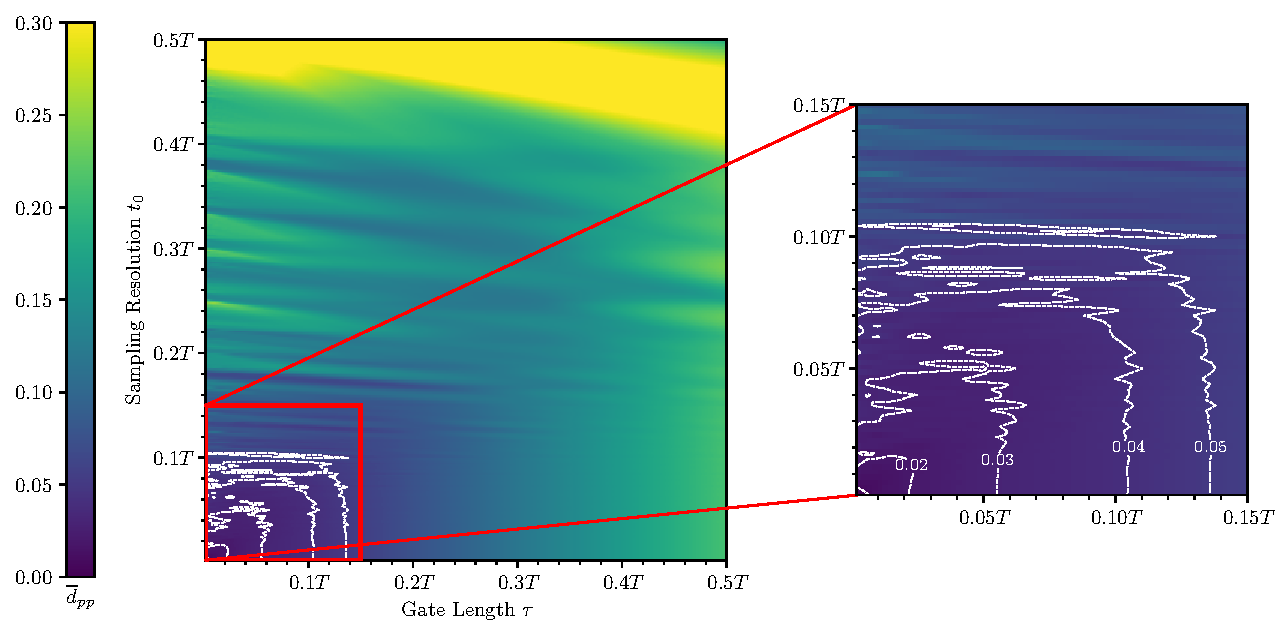
\includegraphics[width=0.75\textwidth]{Figures/Combinations/square_real.pdf}
	\caption{Two-dimensional plots showcasing the $m$ different deviations $\overline{d}_{pp}$ of the square wave signal for different combinations of gate length $\tau$ and sampling resolution $t_0$, where both parameters are set to $\tau, t_0 \in \interval[scaled, open left]{0}{0.5T}$, with dashed contour lines for $\overline{d}_{pp} = 0.01, \dotsc ,0.05$.}
	\label{fig:square-real-combination}
\end{figure}
\subsubsection{Bat-Signal} \label{sssec:Bat-Signal}
In order to test the validity of the self-developed method regarding complicated signals with rapid and frequent changes in amplitude, as they often occur in physical processes and measurements, the same temporal discretization and deviation evaluation can be applied to a more complicated Bat-Signal (\cref{fig:batman-real-i500-s250}). The deviation $\overline{d}_{pp}$ for $m$ different combinations of gate length $\tau$ and sampling resolution $t_0$ can be calculated and plotted in two dimensions in much the same way, resulting in \cref{fig:batman-real-combination}. It is apparent that the same deviation of $\overline{d}_{pp} < 5\%$ requires even lower values for the parameters (i.\,e. a gate length of $\tau < 0.1T$ and a sampling resolution of $t_0 < 0.05T$). This also means that those parameters, which are easily within experimental feasibility, yield a deviation of $\overline{d}_{pp} \approx 5\%$, which is not only around four times higher than the sine wave signal, but also around one-fourth to one-third higher than the deviation of the square wave signal.
\begin{figure}[H]
	\centering
	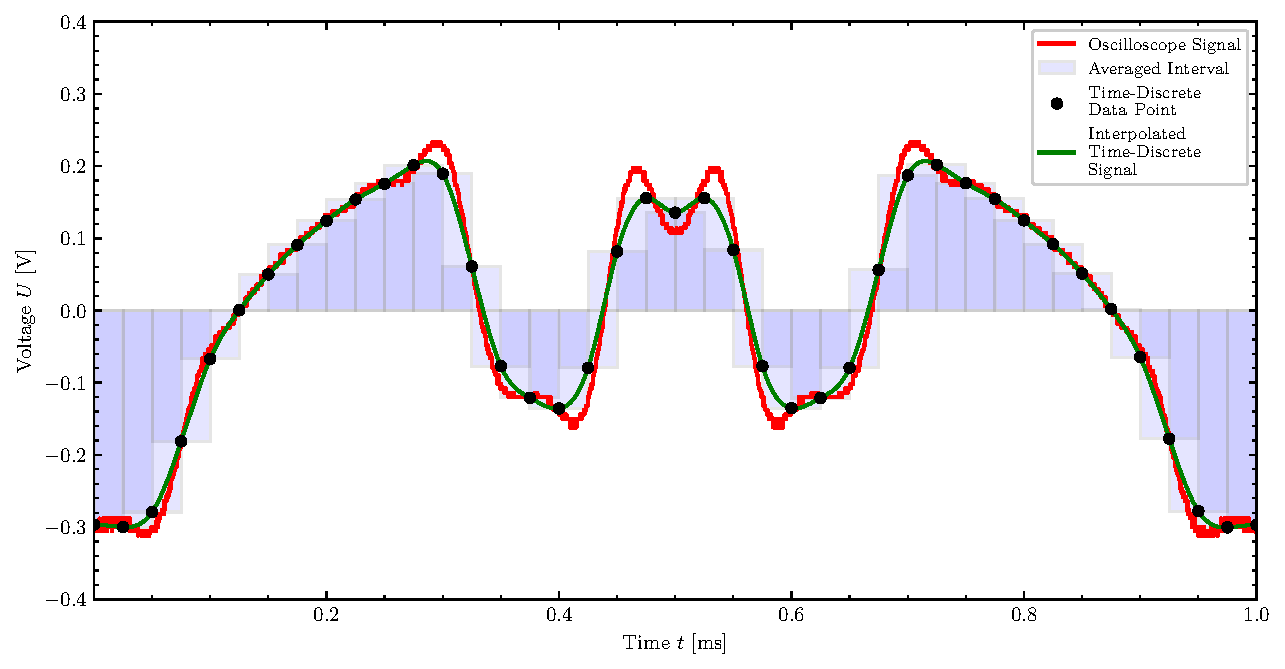
\includegraphics[width=0.75\textwidth]{Figures/Signals/batman_real_i500_s250.pdf}
	\caption{Plot of the oscilloscope Bat-Signal $U\left(t\right)$ along with the (overlapping) intervals over whom are averaged, the time-discrete data points $\overline{U}_j\left(t_{g_j}\right)$ and the interpolated time-discrete signal $U_S\left(t\right)$ for a gate length of $\tau = 0.05T$ and a sampling resolution of $t_0 = 0.025T$.}
	\label{fig:batman-real-i500-s250}
\end{figure}
The Bat-Signal is a perfect example of a complicated signal with rapid changes in amplitude and slope. The signal not only features sections with little change in trend, but also those of sharp and sudden rise or decline (such as the spikes around the middle). It is these areas where the attenuating effect of the averaging approach to the amplitude is particularly apparent, especially with increasing gate length $\tau$.
\begin{figure}[H]
	\centering
		\centering
	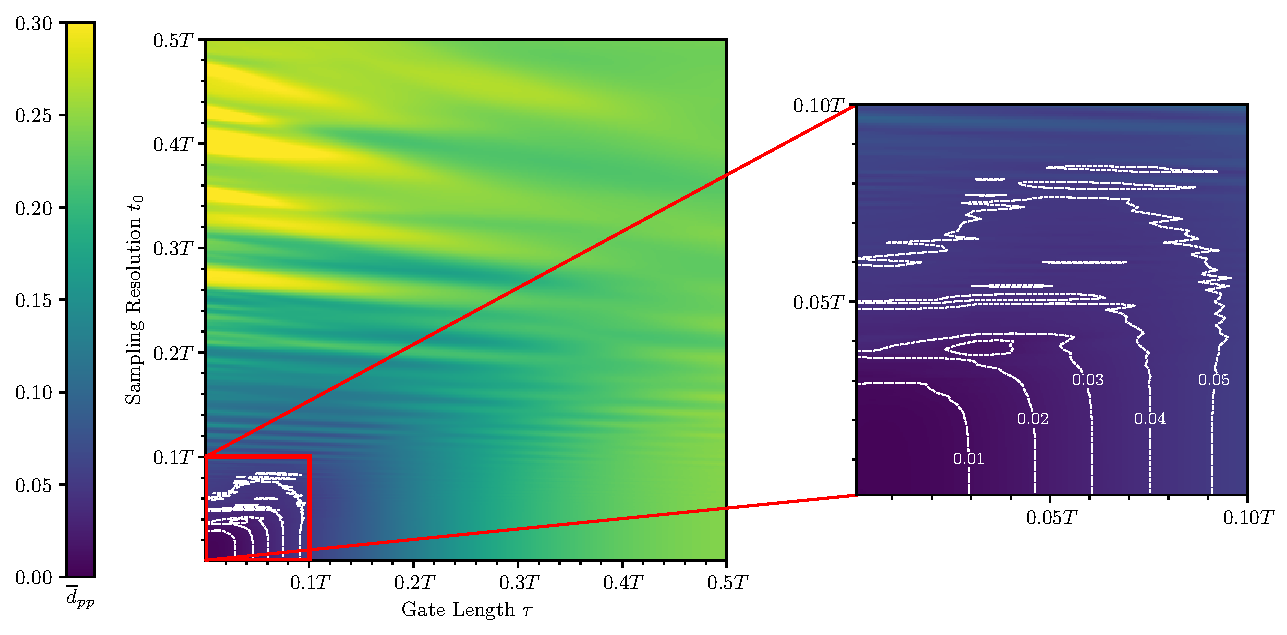
\includegraphics[width=0.75\textwidth]{Figures/Combinations/batman_real.pdf}
	\caption{Two-dimensional plots showcasing the $m$ different deviations $\overline{d}_{pp}$ of the Bat-Signal for different combinations of gate length $\tau$ and sampling resolution $t_0$, where both parameters are set to $\tau, t_0 \in \interval[scaled, open left]{0}{0.5T}$, with dashed contour lines for $\overline{d}_{pp} = 0.01, \dotsc ,0.05$.}
	\label{fig:batman-real-combination}
\end{figure}
\subsection{Discussion} \label{ssec:implementation-discussion}
The previous sections presented a method to investigate the inherent discretization deviations of time-resolved measurement processes. This especially allows the prediction of suitable measurement parameters $\tau$ and $t_0$ within specified error limits for different dynamic processes (represented by the input signal $U\left(t\right)$). With the temporal discretization step, the measurement process of time-resolved methods (e.\,g. interference gating) could be reproduced exactly, which is a direct implementation of the experiment.

Interpolating the $n$ time-discrete data points with a cubic spline $S \in C^2$ further allows for a comparison of signals with different length or sampling resolution, whereas normalizing the deviation $\overline{d}$ to the peak-to-peak amplitude $U_{pp}$ ensures applicability for values that are (near) zero without numerical instability. Another advantage of the normalized deviation $\overline{d}_{pp}$ is the ability to compare different physical processes with non-matching amplitude $U_{pp}$.

The self-developed method was applied to three different signals, namely a sine wave, square wave and Bat-Signal, in \cref{ssec:real-signals}. Comparing all three signals shows that the gate length $\tau$ and sampling resolution $t_0$ required to achieve a representative output from the interference gating method (i.\,e. a deviation $\overline{d}_{pp}$ of up to $5\%$) is highly dependent on the oscilloscope signal and varies anywhere from up to $\tau = t_0 \approx 0.3T$ for the sine wave signal to as low as $\tau < 0.1T$ and $t_0 < 0.05T$ for the Bat-Signal.

As described in \cref{ssec:discrete-signals}, signals can also be analyzed in the frequency domain $f$ instead of the time domain $t$, as is common in signal theory. As an example, this approach is made for the Bat-Signal to separate it into its frequency components, along with the interpolated time-discrete signal for gate length $\tau$ and sampling resolution $t_0$ set to $\tau = t_0 = 0.1T, \dotsc ,0.5T$, and display the result as a bar plot (\cref{fig:batman-dft}).

Due to its complicated composition, the Bat-Signal features a wide array of frequency components with different spectral amplitudes. To be precise, the frequencies ranging from $\SIrange{1}{5}{\kilo\hertz}$ make up the dominant part of the spectrum, while the frequencies ranging from $\SIrange{6}{14}{\kilo\hertz}$ see a steep fall in spectral amplitude. Any frequency components beyond that are only present to a minor degree.

Two particularly interesting observations can be drawn from this discrete Fourier transform:
\begin{itemize}
	\item The lowpass-filtering-effect is especially apparent for the interpolated time-discrete signals. Whereas a gate length $\tau$ and sampling resolution $t_0$ of $\tau = t_0 = 0.1T$ still yield frequency components of up to $\SI{7}{\kilo\hertz}$, other parameters of $\tau = t_0 = 0.2T, \dotsc ,0.5T$ have a cutoff frequency of $\SI{3}{\kilo\hertz}$.
	\item The change in spectral amplitude $Q$ for different gate lengths $\tau$ and sampling resolutions $t_0$ does not follow any concrete correlation or pattern.
\end{itemize}
\begin{figure}[H]
	\centering
	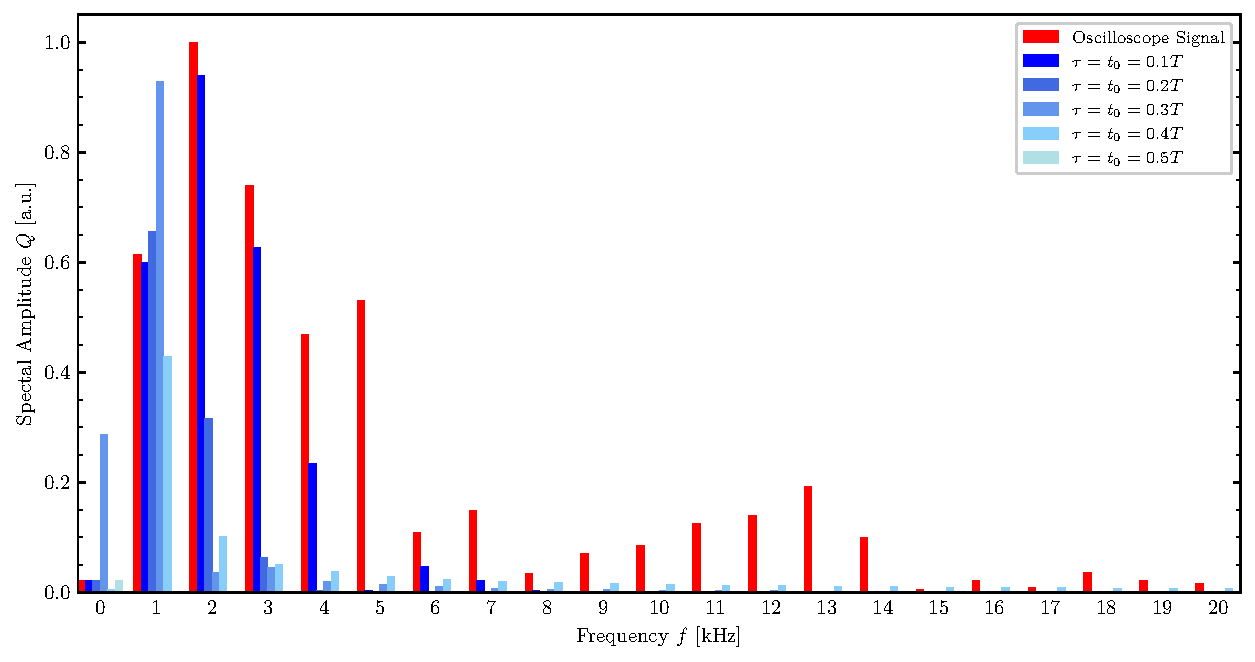
\includegraphics[width=0.75\textwidth]{Figures/Signals/batman_dft.pdf}
	\caption{Bar plot representing the frequency spectrum of the Bat-Signal using the discrete Fourier transform for the oscilloscope signal $U\left(t\right)$ as well as different interpolated time-discrete signals $U_S\left(t\right)$ with the gate length $\tau$ and sampling resolution $t_0$ set to $\tau = t_0 = 0.1T, \dotsc ,0.5T$.}
	\label{fig:batman-dft}
\end{figure}
It can be drawn from this that a quantitative comparison of different signals in the frequency domain is hardly possible for complicated signals that are made up of a wide array of frequency components. This shows that the self-developed deviation evaluation method in the time domain introduced in \cref{ssec:evaluation-method} is able to quantify the deviation of such discretization approaches, as used by the interference gating method, for arbitrary combinations of gate length $\tau$ and sampling resolution $t_0$, while still being suitable for a wide range of signals, and should thus be the preferred method.

While the results obtained seem promising at first, especially with respect to the prediction of suitable measurement parameters $\tau$ and $t_0$, their validity needs to be verified. For this purpose, comparisons with phase slopes of time-resolved, reconstructed electron waves are established in \cref{sec:application}. 
\newpage
\section{Application} \label{sec:application}
In order to test the self-developed deviation evaluation method from the previous \cref{sec:implementation}, the following section presents the experimental setup used to acquire dynamic phases of time-resolved electron waves for a specific set of gate length $\tau$ and sampling resolution $t_0$, derive their slopes and compare them to the time-discrete data points for the three previously detailed signals.
\subsection{Experiment} \label{ssec:application-experiment}
All measurements\footnote{Due to the COVID-19 pandemic, all measurements and pictures were graciously provided by the supervisor.} were done with the FEI Titan™ 80-300 Berlin Holography Special TEM (\cref{fig:FEI-Titan}) in a special extended Lorentz holography mode \cite{Wagner2019}. All holograms for the coplanar capacitor (\cref{fig:EH-biased}), which was cut from a micro-electro-mechanical system (MEMS) chip with a FEI Helios NanoLab™ 600 and placed in a DENSsolution Wildfire™ S3 In Situ TEM Heating System (\cref{fig:TEM-Holder}), were captured with a Gatan UltraScan™ 1000 CCD Camera for an exposure time $T_{exp}$ and an acceleration voltage $U_a$. The capacitor was externally biased with $U_{ext}$ and measurements with $U_{ext} = \SI{0}{\volt}$ were used as empty holograms. A GW Instek™ GDS-1102B Digital Oscilloscope was used to monitor the applied signal.
\begin{figure}[H]
	\centering
	\begin{subfigure}[c]{\textwidth}
		\centering
		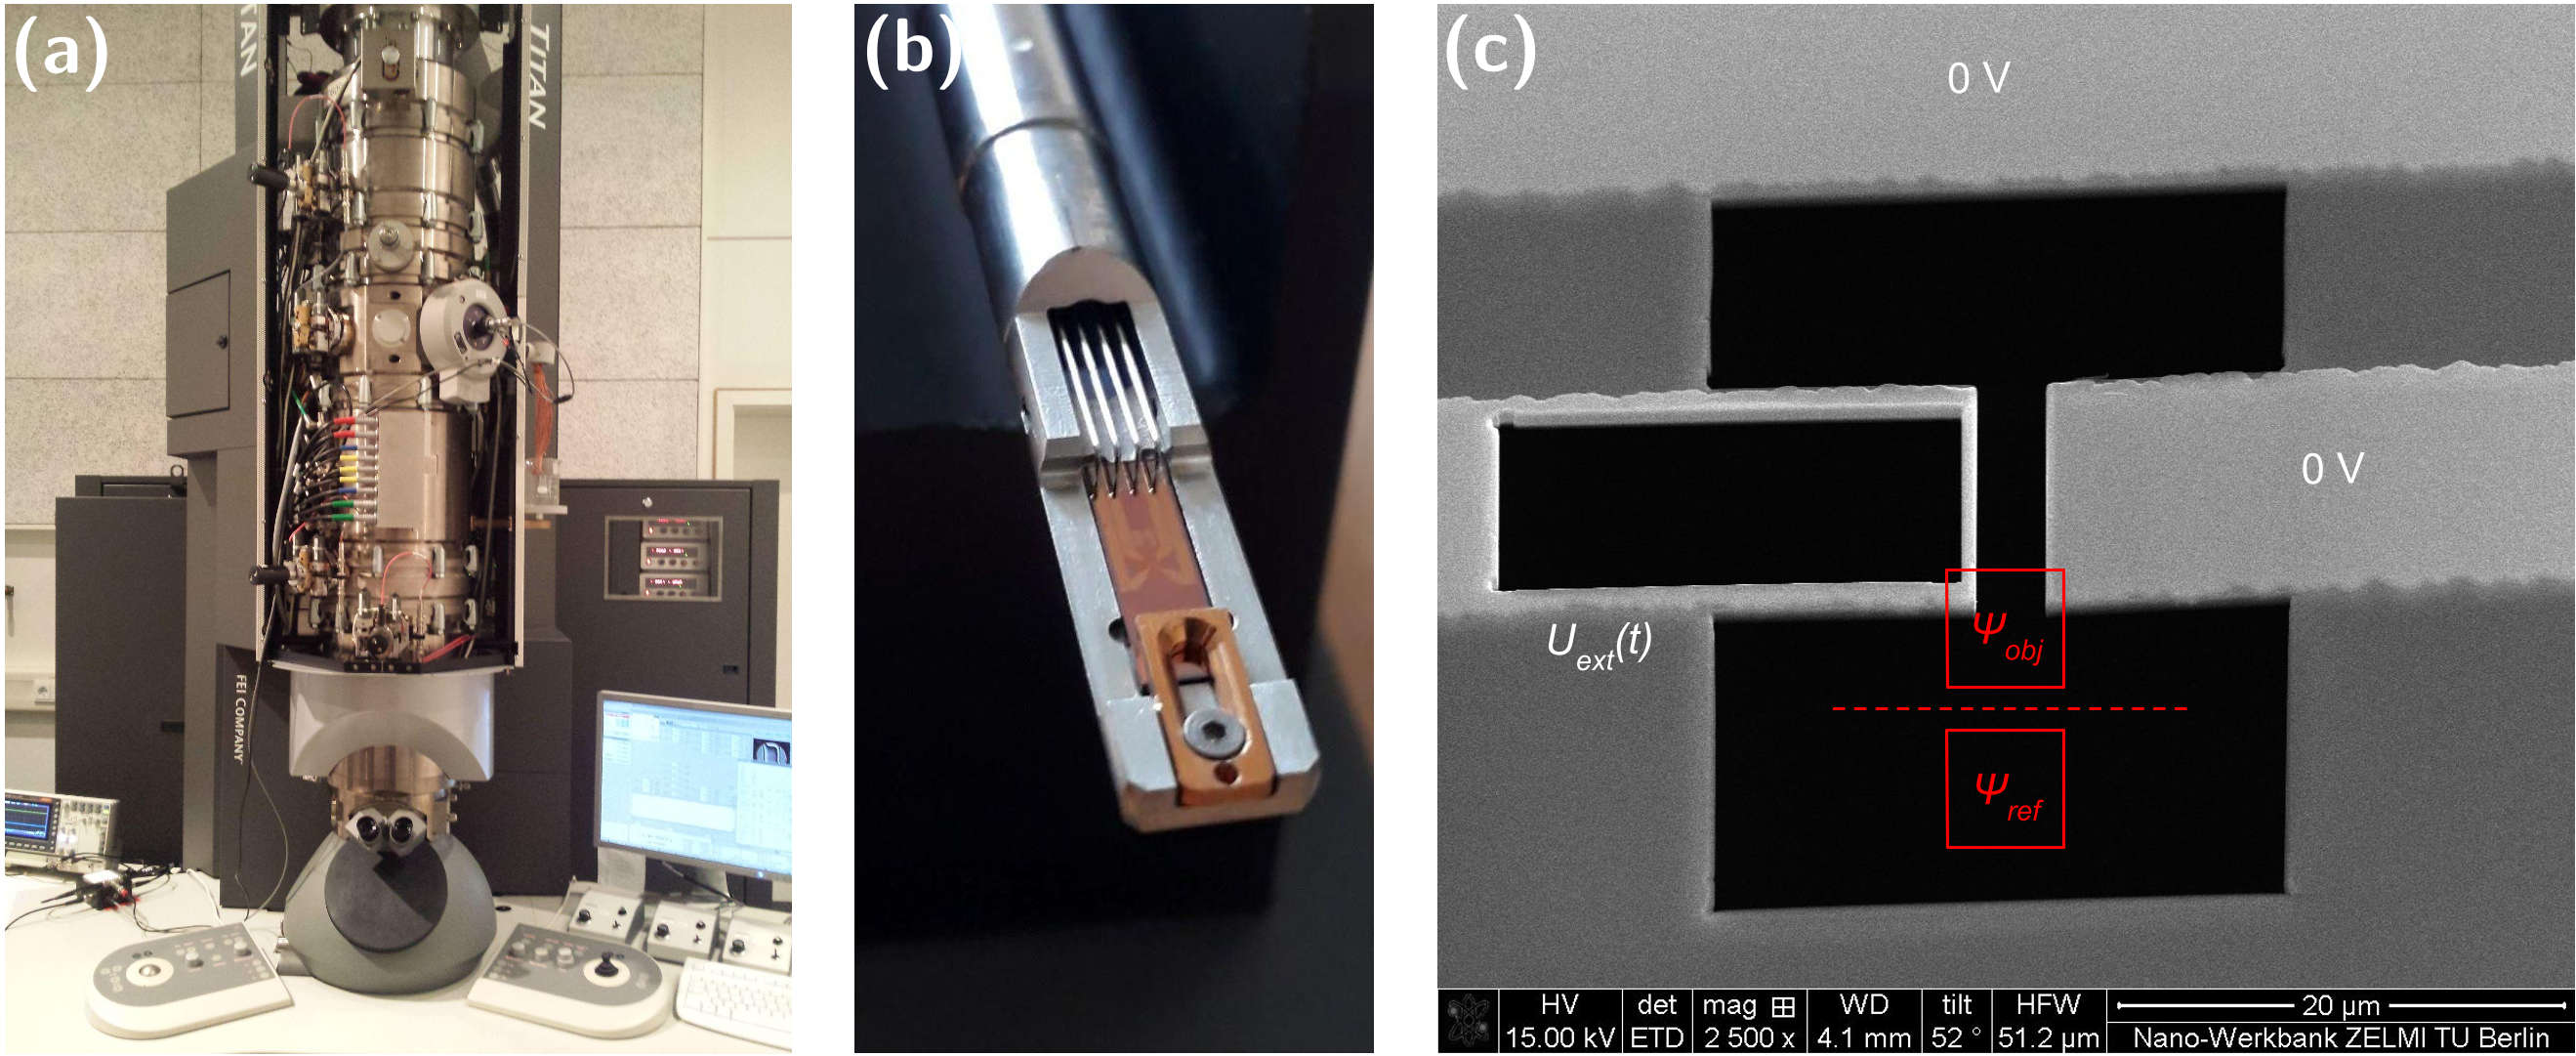
\includegraphics[width=\textwidth]{Figures/Setup.pdf}
		\phantomsubcaption
		\label{fig:FEI-Titan}
	\end{subfigure}%
	\begin{subfigure}[c]{0\textwidth}
		\centering
		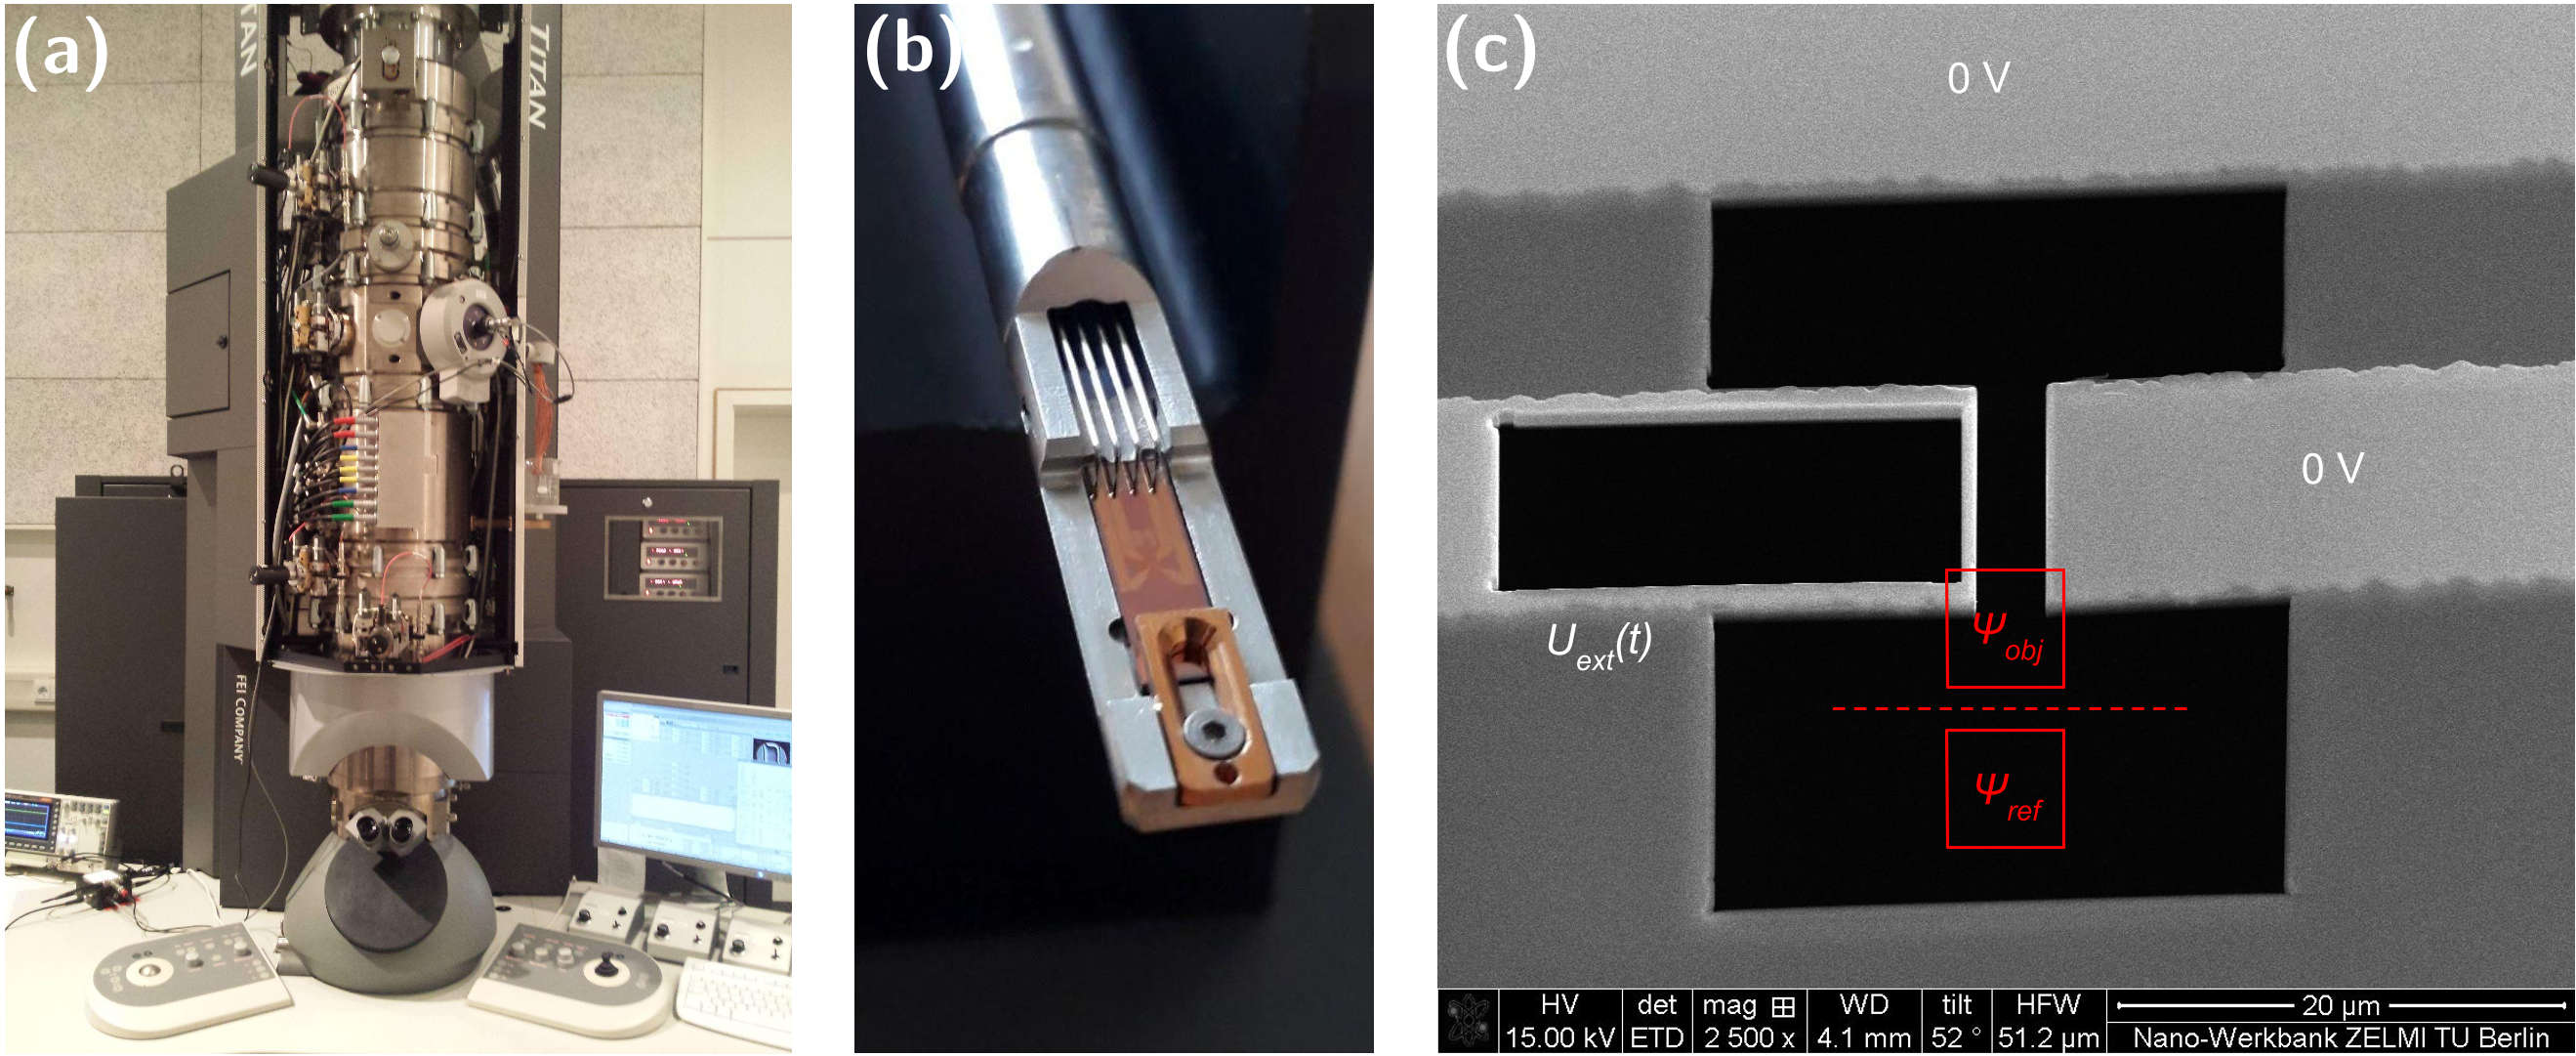
\includegraphics[width=\textwidth]{Figures/Setup.pdf}
		\phantomsubcaption
		\label{fig:TEM-Holder}
	\end{subfigure}%
	\begin{subfigure}[c]{0\textwidth}
		\centering
		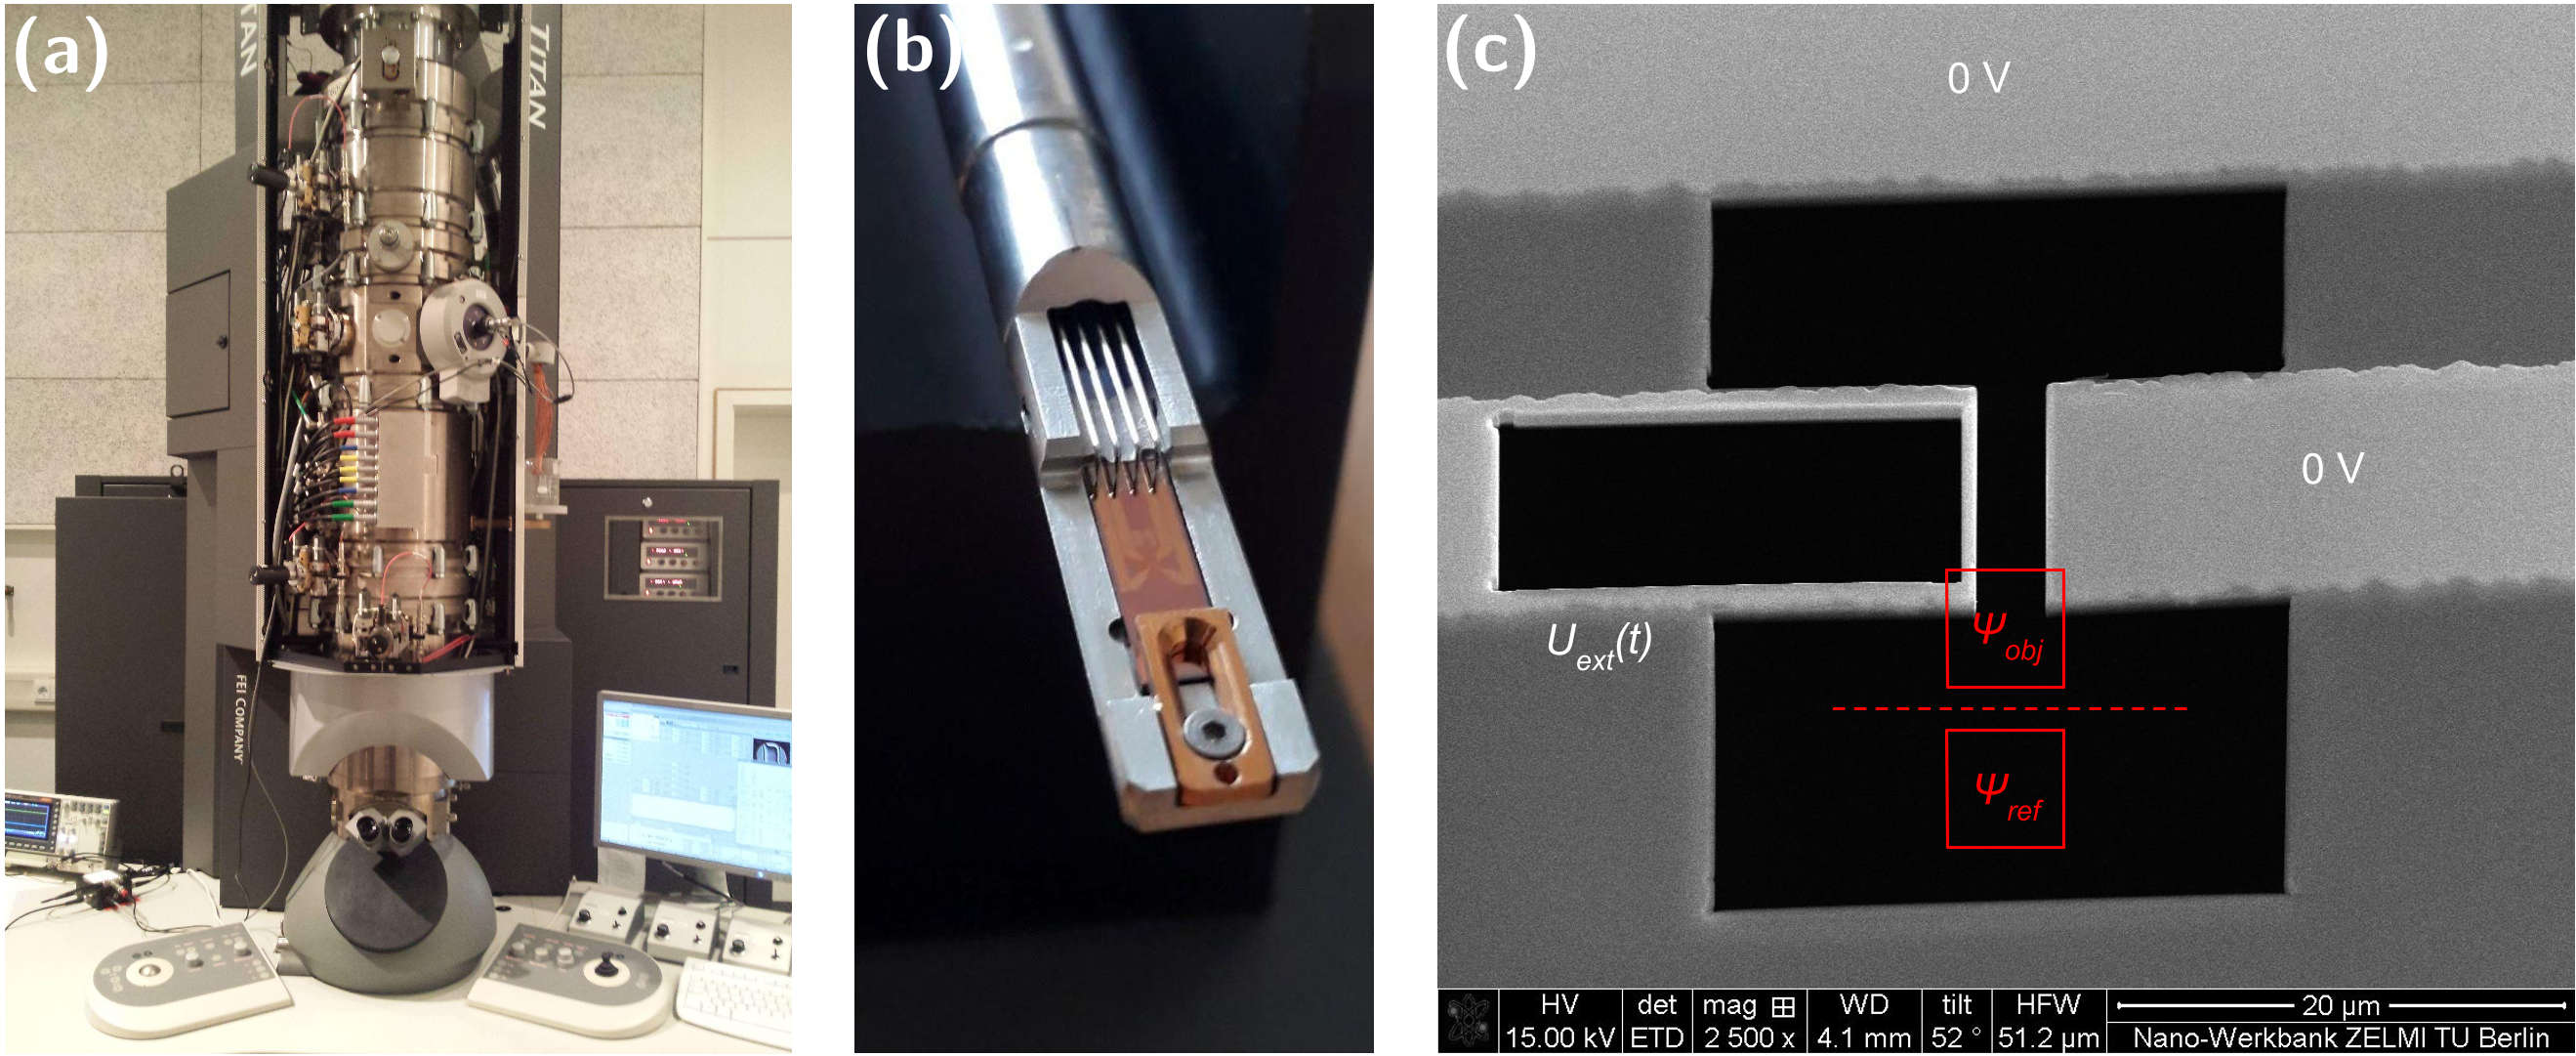
\includegraphics[width=\textwidth]{Figures/Setup.pdf}
		\phantomsubcaption
		\label{fig:Capacitor-SEM}
	\end{subfigure}%
	\caption{Experimental setup featuring the (a) FEI Titan™ 80-300 Berlin Holography Special TEM, (b) DENSsolution Wildfire™ S3 In Situ TEM Heating System and (c) SEM micrograph of the coplanar capacitor with the position of the biprism (dashed line) marked for the respective electron holography setup.}
	\label{fig:Experiment-Setup}
\end{figure}
By using focused ion beam milling, the required capacitor can be manufactured from a MEMS chip by cutting through a conductive trace and milling a window into the adjacent silicon nitride diaphragm. Both ends of the severed trace, which is made of a $\SI{200}{\nano\metre}$ thick Au layer covered in $\SI{200}{\nano\metre}$ thick Si\textsubscript{3}Ni\textsubscript{4} layers, make up the terminals of the capacitor (\cref{fig:Capacitor-SEM}) with a distance of $\SI{2.75}{\micro\metre}$ in between and a width of $\SI{15}{\micro\metre}$.

Then, the capacitor is placed in an in situ TEM holder, which provides a mechanical and electrical connection using spring contacts and a cooper latch (\cref{fig:TEM-Holder}).

Biasing the left terminal with the external voltage $U_{ext}$ while grounding the right terminal leads to a capacitor with a one sided potential that varies between $+U_{ext}$ and $-U_{ext}$ for an AC voltage source (\cref{fig:Capacitor-SEM}). The electric potential of the capacitor leads to a modulation of the phase $\varphi\left(\vb{r}\right)$ regarding the image wave ${\psi}_{rec}\left(\vb{r}\right)$ \cite{Niermann2017}.

In order to improve the signal-to-noise ratio, multiple holograms with $U_{ext} = \text{const}$ are captured and then averaged for every gate position $t_{g_j}$. The phase slope $\dv*{}{x} \varphi\left(x\right)$, which is proportional to the external voltage $U_{ext}$, is calculated by defining a rectangular area in between both terminals of the capacitor, determining the gradient through the distance of adjacent pixels and projecting it onto the connecting vector going from the grounded terminal to the biased one. The error of the phase slope follows by calculating the variance.
\subsection{Results} \label{ssec:application-results}
With the phase slope being proportional to the capacitor voltage (i.\,e. $\dv*{}{x} {\varphi}_{t_{g_j}}\left(x\right) \sim U_{ext}\left(t_{g_j}\right)$), the question of direct comparison to the oscilloscope signal $U\left(t\right)$ arises.

Starting with the sine wave signal, where the measurement uses an acceleration voltage of $U_a = \SI{300}{\kilo\volt}$, an exposure time of $T_{exp} = \SI{3}{\second}$ each and averages five consecutive holograms, as well as a gate length of $\tau = 0.1T$ and sampling resolution of $t_0 = 0.05T$ for both the phase slopes and the time-discrete data points, both $\dv*{}{x} {\varphi}_{t_{g_j}}\left(x\right)$ and $\overline{U}_j\left(t_{g_j}\right)$ constitute an accurate representation of the oscilloscope signal (\cref{fig:sine-slope}). Not only do all values for the phase slope have little to no deviation from the time-discrete points, but the attenuating effect of the temporal discretization on the amplitude is also non-present for the specified parameters.
\begin{figure}[H]
	\centering
	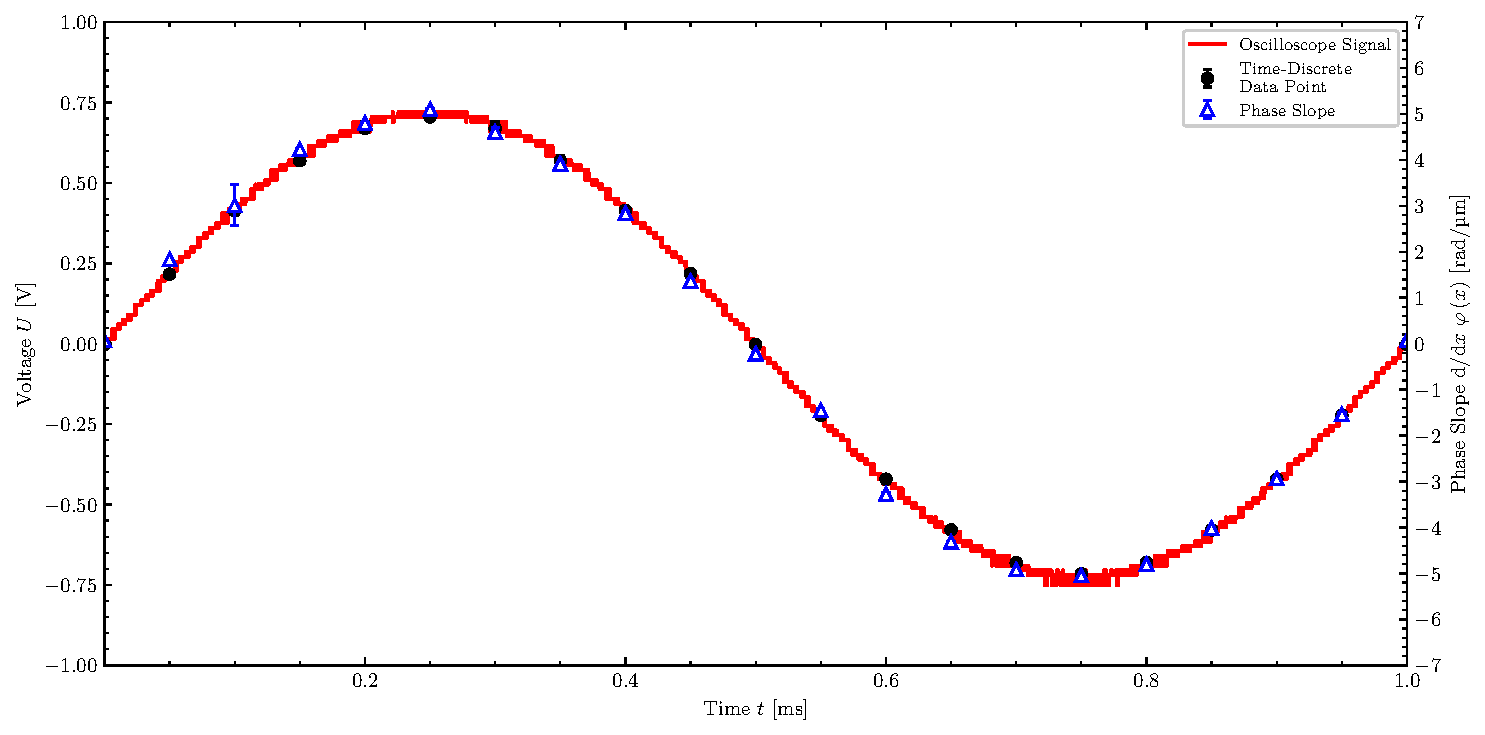
\includegraphics[width=0.75\textwidth]{Figures/Slope/sine_slope.pdf}
	\caption{Plot of the oscilloscope sine wave signal $U\left(t\right)$ along with the phase slopes $\dv*{}{x} \varphi\left(x\right)$ at $t_{g_j}$ and the time-discrete data points $\overline{U}_j\left(t_{g_j}\right)$ for a gate length of $\tau = 0.1T$ and a sampling resolution of $t_0 = 0.05T$.}
	\label{fig:sine-slope}
\end{figure}
The same measurement of the phase slopes $\dv*{}{x} \varphi\left(x\right)$, with a gate length $\tau = 0.1T$ and a sampling resolution of $t_0 = 0.05T$, can be done for the square wave signal (\cref{fig:square-slope}). Here, the acceleration voltage is set to $U_a = \SI{200}{\kilo\volt}$ with an exposure time of $T_{exp} = \SI{4}{\second}$ each for four consecutive holograms that are averaged.

Similar to the sine wave signal from above, both the phase slopes and the time-discrete data points provide an accurate representation of the oscilloscope square wave signal. The only noticeable deviations between the phase slopes and the time-discrete data points occur during the rise/fall time of the oscilloscope signal, where the phase slope is either almost identical to the oscilloscope signal and the time-discrete data point deviates, or both the phase slope and the time-discrete data point feature a similar deviation from the oscilloscope signal. It can be observed, however, that the measured phase slopes feature a phase wedge, which in turn causes $\abs*{\dv*{}{x} {\varphi}_{t_{g_j}}\left(x\right)}$ to be non-symmetric around zero. Furthermore, the oscilloscope signal features a plateau during the rise/fall time with a width of $\approx \SI{0.15}{\micro\second}$.

The discharge of the capacitor can be modeled using the exponential function \cite{carr2001}: $$U\left(t\right) = U_{pp} \cdot e^{-\frac{t}{R\cdot C}}$$ and the measured capacitance $C$ and resistance $R$. Connecting an ohmmeter directly to the MEMS chip prior to cutting through the conductive trace allows for a measurement of the resistance with $R = \SI{392 \pm 20}{\ohm}$, while a Keysight™ E4980A Precision LCR Meter can be used to measure the capacitance at $C = \SI{152 \pm 20}{\pico\farad}$ in a frequency range of $\SIrange{70}{700}{\kilo\hertz}$ \cite{Wagner2018}.
\begin{figure}[H]
	\centering
	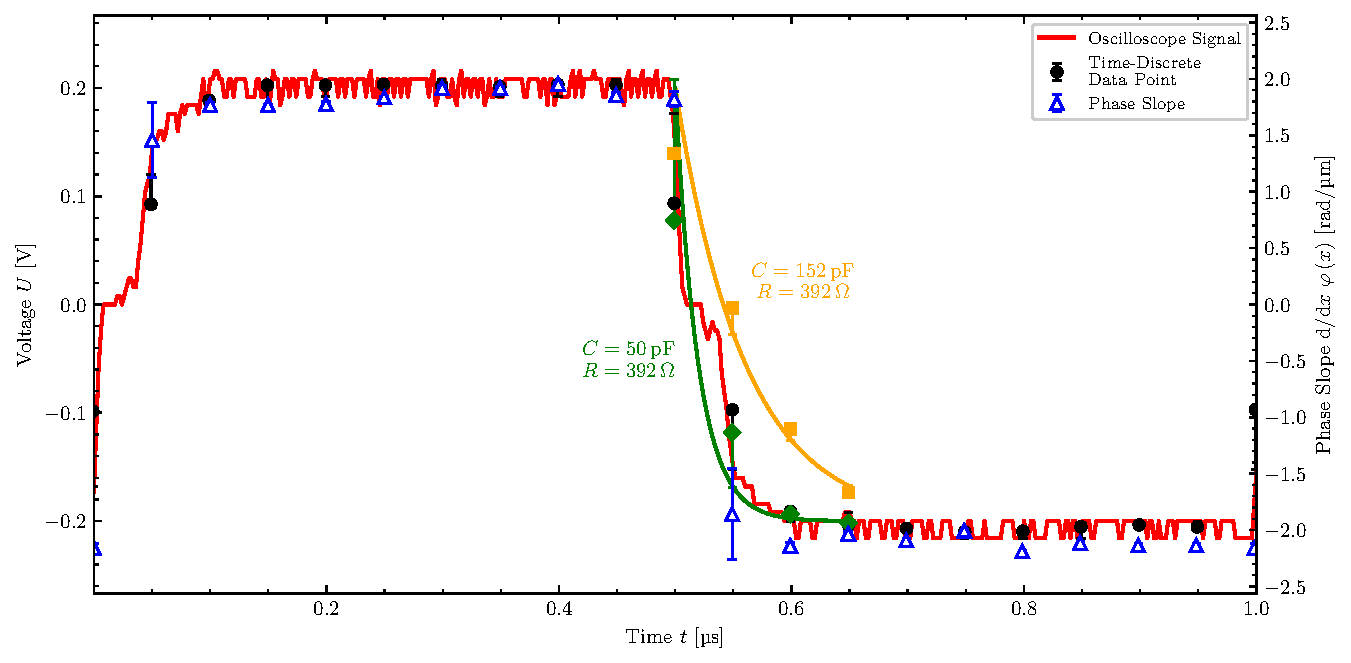
\includegraphics[width=0.75\textwidth]{Figures/Slope/square_slope.pdf}
	\caption{Plot of the oscilloscope square wave signal $U\left(t\right)$ along with the phase slopes $\dv*{}{x} \varphi\left(x\right)$ at $t_{g_j}$ and the time-discrete data points $\overline{U}_j\left(t_{g_j}\right)$ for a gate length of $\tau = 0.1T$ and a sampling resolution of $t_0 = 0.05T$. Moreover, an exponential function can be used for the discharge of the capacitor between $\SI{0.5}{\micro\second}$ and $\SI{0.65}{\micro\second}$ to demonstrate the fall time for different capacitances $C$ and constant resistance $R$.}
	\label{fig:square-slope}
\end{figure}
With these parameters, it is apparent that the modeled curve is falling too slow to approximate the capacitor, causing the time-discrete data points from $\SIrange{0.55}{0.65}{\micro\second}$ to distance themselves from the phase slopes. Assuming the capacitance at $C =\SI{50}{\pico\farad}$ causes the resulting time-discrete data points to move closer to the phase slopes.

At last, the same measurement of the phase slopes $\dv*{}{x} \varphi\left(x\right)$, with a gate length $\tau = 0.1T$ and a sampling resolution of $t_0 = 0.05T$, can be done for the Bat-Signal (\cref{fig:batman-slope}). Here, the acceleration voltage is set to $U_a = \SI{300}{\kilo\volt}$ with an exposure time of $T_{exp} = \SI{3}{\second}$ each for five consecutive holograms that are averaged, identical to the square wave signal.
\begin{figure}[H]
	\centering
	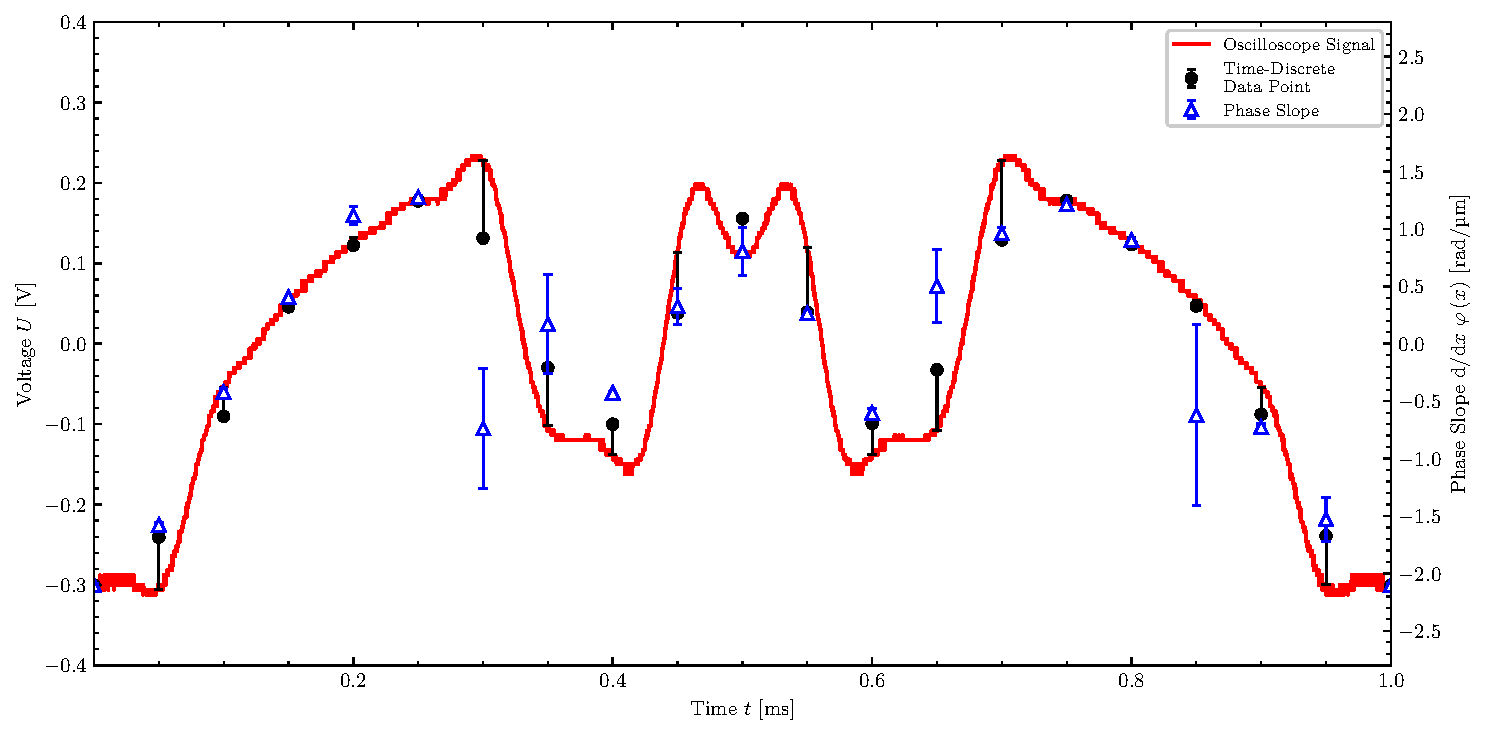
\includegraphics[width=0.75\textwidth]{Figures/Slope/batman_slope.pdf}
	\caption{Plot of the oscilloscope Bat-Signal $U\left(t\right)$ along with the phase slopes $\dv*{}{x} \varphi\left(x\right)$ at $t_{g_j}$ and the time-discrete data points $\overline{U}_j\left(t_{g_j}\right)$ for a gate length of $\tau = 0.1T$ and a sampling resolution of $t_0 = 0.05T$.}
	\label{fig:batman-slope}
\end{figure}
The complicated Bat-Signal, with its rapid changes in amplitude and slope along with the symmetry of the signal, features a wider array of deviations between the phase slopes, the time-discrete data points and the oscilloscope signal. The areas of steady rise or decline (i.\,e. $\SIrange{0}{\approx 0.3}{\milli\second}$ and $\SIrange{\approx 0.7}{1.0}{\milli\second}$) feature only small deviations between the phase slopes and the time-discrete data points, with both of them bordering on the oscilloscope signal. The phase slopes for $t_{g_j} = \SI{0.3}{\milli\second}$ and $t_{g_j} = \SI{0.85}{\milli\second}$ show major deviations from the time-discrete data points, which are neighboring the oscilloscope signal. Furthermore, the sections of sharp rise or decline (i.\,e. $\SIrange{\approx 0.3}{\approx 0.4}{\milli\second}$ and $\SIrange{\approx 0.6}{\approx 0.7}{\milli\second}$) show less deviation between the phase slopes and time-discrete data points than between the phase slopes and the oscilloscope signal, adhering to the above established presumption of the phase slopes being closer to the time-discrete data points. The middle section of the signal featuring the spikes (i.\,e. $\SIrange{\approx 0.4}{\approx 0.6}{\milli\second}$) shows the same behavior, with the exception of the phase slope located at exactly the middle of the signal (i.\,e. $t_{g_j} = \SI{0.5}{\milli\second}$), for which the phase slope is closer to the oscilloscope signal than to the time-discrete data point.
\subsection{Discussion} \label{ssec:application-discussion}
The sine wave signal, being the simplest case to measure, shows little to no deviation of both the phase slopes and the time-discrete data points from the oscilloscope signal for a gate length of $\tau = 0.1T$ and a sampling resolution of $t_0 = 0.05T$. Therefore, the comparison between the phase slopes and the oscilloscope signal can be made without further considerations, as predicted by the self-developed method.

The square wave signal, however, features deviations during the rise/fall time of the oscilloscope signal where the capacitor is (dis-)charging. Here, the plateau with a width of $\approx \SI{0.15}{\micro\second}$ is caused by both capacitive reflections on the conductive tracks and cables \cite{carr2001} and parasitic capacitances on the MEMS chip \cite{Wagner2018}.

The large error of the measured resistance $R$ and capacitance $C$ can likewise be attributed to the above mentioned parasitic capacitances and is depended on the thickness of the silicon nitride layer \cite{Wagner2018}. Nevertheless, the higher agreement of the exponential model for a capacitance of $C = \SI{50}{\pico\farad}$ with the oscilloscope signal, therefore causing the resulting time-discrete data points to move closer to the measured phase slopes, shows that the measured capacitance of $C = \SI{152 \pm 20}{\pico\farad}$ is more applicable to the whole MEMS chip rather than the single capacitor investigated. The deviation between the time-discrete data point and the phase slope at $t_{g_j} = \SI{0.5}{\micro\second}$ is due to \emph{overshooting}, an effect that only applies to the single capacitor, therefore only effecting the phase slope, instead of the whole MEMS chip \cite{Stewart2006}. This also shows that the interference gating method is an excellent candidate for measurements of single electronic components inside sophisticated circuits.

The deviations between the phase slopes, the time-discrete data points and the oscilloscope Bat-Signal are highly dependent on the measured section of the signal. The non-symmetric deviations of the phase slope for $t_{g_j} = \SI{0.3}{\milli\second}$ and $t_{g_j} = \SI{0.85}{\milli\second}$ can be attributed to a measurement error in the empty hologram caused by external fields. The deviation of the phase slope between the spikes of the signal is caused by high-frequency components, showing that a gate length of $\tau = 0.1T$ is pushing the limits of accurate representation. Furthermore, changes that are smaller than $0.5\tau$, such as narrow spikes in the signal, contribute to a large deviation of both the phase slopes and the time-discrete data points from the oscilloscope signal. Overall, both the phase slopes and the time-discrete data points still amount to a fairly accurate representation of the oscilloscope signal when selecting a gate length of $\tau = 0.1T$ and a sampling resolution of $t_0 = 0.05T$.

Following the above made observations, the temporal discretization based deviations of the interference gating method can be regarded as a lower bound error that is, regardless of experimental setup, always present. Therefore, the phase slopes are not only proportional, but also closer to the time-discrete data points (i.\,e. $\dv*{}{x} {\varphi}_{t_{g_j}}\left(x\right) \sim \overline{U}_j\left(t_{g_j}\right)$) than to the oscilloscope signal. Since perfect measurements are not feasible to achieve, various deviations that arise from different measurement errors have to be accounted for in addition to this lower bound error.
\newpage
\section{Summary and Outlook} \label{sec:summary-outlook}
The aim of this thesis was to develop and test a suitable method for the quantitative analysis of deviations caused by temporal discretization of signals as they appear in time-resolved investigations.

In order to place this task in the correlated scientific setting, and after a brief motivation in \cref{sec:introduction}, the theoretical backgrounds of related fields were introduced in \cref{sec:theoretical-foundations}.

In \cref{sec:implementation} the self-developed method for quantitative analysis of deviations due to temporal discretization of signals was presented and its application to three different types of signals (sine wave, square wave and Bat-Signal) was discussed. The temporal discretization and deviation evaluation method can be broken down into two main steps: The first step deals with the actual discretization of the input signal by splitting it into intervals of equal length, the so-called gate length $\tau$, and equal spacing, the so called sampling resolution $t_0$, and averaging over them, whereas the second step evaluates the deviation between the time-discrete and input signal at every data point by means of a cubic spline. Setting the gate length to $\tau = 0.1T$ and the sampling resolution to $t_0 = 0.05T$ results in an averaged and normalized deviation $\overline{d}_{pp}$ that varies anywhere between $\overline{d}_{pp} < 1\%$ for the sine wave signal and $\overline{d}_{pp} \approx 5\%$ for the Bat-Signal. Furthermore, inspecting the Bat-Signal in the frequency domain $f$ instead of the time domain $t$ shows that the self-developed method delivers a more intuitive and quantified approach for complicated signals compared to common signal-theoretical methods for the determination of discretization based deviations.

For experimental comparison, discretized phase slopes of time-resolved electron waves, which were obtained via time-resolved electron holography by interference gating, were examined in \cref{sec:application}. The measured phase slopes for the sine wave signal showed little to no deviation to the time-discrete data points of the oscilloscope signal. In comparison, the square wave signal featured only small deviations between the measured phase slopes and the time-discrete data points during the polarity change of the input signal, which can be attributed to parasitic capacitances and described, in combination with the self-developed method, using a modeling approach, drawing a connection to real physical effects. In detail, the exponential curve initially failed to approximate the oscilloscope signal using the measured capacitance $C = \SI{152 \pm 20}{\pico\farad}$ of the MEMS chip, whereas assuming the capacitance at $C = \SI{50}{\pico\farad}$ resulted in a higher agreement between them, showing that the measured capacitance is more applicable to the whole MEMS chip rather than the single capacitor investigated. At last, the Bat-Signal showed a similar behavior of small deviations between the phase slopes and the time-discrete data points, except for a few asymmetric deviations due to stray fields.

In particular, comparison with experimental data has shown that the self-developed method is a promising approach for quantitative analysis of temporal discretization based deviations. Moreover, quantitative calculations show that the interference gating method along with a gate length of $\tau = 0.1T$ and a sampling resolution of $t_0 = 0.05T$, which is easily within experimental feasibility, is able to sample simplified signals, such as a sine or square wave, with little to no deviation.

The presented method therefore allows for a smart choice of gate length $\tau$ and sampling resolution $t_0$ for future investigations and thus contributes to increasing the efficiency of time-resolved electron-holographic measurements and enabling significant time savings in the measurement process. Furthermore, a deeper investigation of the possibility to describe deviations by means of modeling, in connection with the self-developed method (as in the case of the (dis-)charging capacitor), seems particularly interesting and opens the door for quantitative investigation of dynamic physical processes.
\newpage

\printbibliography[heading=bibintoc]
\newpage

\appendix
\section{Source Code}
The following implementation uses the \textsc{python} programming language to split the input signal into equally sized and spaced intervals:
\begin{minted}[xleftmargin=\svtheparindent\relax,linenos,breaklines,frame=single,fontsize=\footnotesize]{python}
from scipy.interpolate import CubicSpline
from more_itertools import windowed
from tqdm.contrib import tzip
import numpy as np

def split(data_x, data_y, interval_size, step_size, period_length, pp_amplitude, iterate=False):
	x_split = [[x for x in val if x is not None] for val in list(windowed(data_x, interval_size, step=step_size))]
	y_split = [[y for y in val if y is not None] for val in list(windowed(data_y, interval_size, step=step_size))]

	if len(x_split[-1]) < len(x_split[0]) and not iterate:
		print(f'Warning! Chosen interval size of {interval_size} and step size of {step_size} result in last interval being smaller than the rest.')

	result = np.vstack([np.array([np.average(val_x), np.average(val_y)]) for (val_x, val_y) in zip(x_split, y_split)])

	spline = CubicSpline(result[:,0], result[:,1])
	spline_dev = [np.abs(val_data - val_spline) for (val_data, val_spline) in zip(data_y[period_length:period_length*2], spline(data_x[period_length:period_length*2]))]

	return x_split, y_split, result, spline, spline(data_x), np.mean(spline_dev)/pp_amplitude

def find_best(data_x, data_y, interval_start, interval_stop, interval_step, step_start, step_stop, step_step, period_length, pp_amplitude):
	combinations = np.zeros(((step_stop - step_start)//step_step + 1, (interval_stop - interval_start)//interval_step + 1))

	for i, a in tzip(range(step_start, step_stop + 1, step_step), range(step_stop - step_start + 1), desc='Steps'):
		for j, b in tzip(range(interval_start, interval_stop + 1, interval_step), range(interval_stop - interval_start + 1), desc='Intervals', leave=False):
			combinations[a,b] = split(data_x, data_y, j, i, period_length, pp_amplitude, iterate=True)[5]

	return combinations
\end{minted}
The function \mintinline{python}{def split()} discretizes the input signal and evaluates the deviation between the interpolated time-discrete signal and the input signal according to the self-developed method described in \cref{sec:implementation}, whereas the function \mintinline{python}{def find_best()} calculates the $m$ different deviations $\overline{d}_{pp}$ for given intervals of gate length $\tau$ and sampling resolution $t_0$ using the above described function.
\end{document}